% Template for PLoS
% Version 2.0 July 2014
%
% To compile to pdf, run:
% latex plos.template
% bibtex plos.template
% latex plos.template
% latex plos.template
% dvipdf plos.template
%
% % % % % % % % % % % % % % % % % % % % % %
%
% -- IMPORTANT NOTE
%
% Be advised that this is merely a template 
% designed to facilitate accurate translation of manuscript content 
% into our production files. 
%
% This template contains extensive comments intended 
% to minimize problems and delays during our production 
% process. Please follow the template 
% whenever possible.
%
% % % % % % % % % % % % % % % % % % % % % % % 
%
% Once your paper is accepted for publication and enters production, 
% PLEASE REMOVE ALL TRACKED CHANGES in this file and leave only
% the final text of your manuscript.
%
% DO NOT ADD EXTRA PACKAGES TO THIS TEMPLATE unless absolutely necessary.
% Packages included in this template are intentionally
% limited and basic in order to reduce the possibility
% of issues during our production process.
%
% % % % % % % % % % % % % % % % % % % % % % %
%
% -- FIGURES AND TABLES
%
% DO NOT INCLUDE GRAPHICS IN YOUR MANUSCRIPT
% - Figures should be uploaded separately from your manuscript file. 
% - Figures generated using LaTeX should be extracted and removed from the PDF before submission. 
% - Figures containing multiple panels/subfigures must be combined into one image file before submission.
% See http://www.plosone.org/static/figureGuidelines for PLOS figure guidelines.
%
% Tables should be cell-based and may not contain:
% - tabs/spacing/line breaks within cells to alter layout
% - vertically-merged cells (no tabular environments within tabular environments, do not use \multirow)
% - colors, shading, or graphic objects
% See http://www.plosone.org/static/figureGuidelines#tables for table guidelines.
%
% For sideways tables, use the {rotating} package and use \begin{sidewaystable} instead of \begin{table} in the appropriate section. PLOS guidelines do not accomodate sideways figures.
%
% % % % % % % % % % % % % % % % % % % % % % % %
%
% -- EQUATIONS, MATH SYMBOLS, SUBSCRIPTS, AND SUPERSCRIPTS
%
% IMPORTANT
% Below are a few tips to help format your equations and other special characters according to our specifications. For more tips to help reduce the possibility of formatting errors during conversion, please see our LaTeX guidelines at http://www.plosone.org/static/latexGuidelines
%
% Please be sure to include all portions of an equation in the math environment, and for any superscripts or subscripts also include the base number/text. For example, use $mathrm{mm}^2$ instead of mm$^2$ (do not use \textsuperscript command).
%
% DO NOT USE the \rm command to render mathmode characters in roman font, instead use $\mathrm{}$
% For bolding characters in mathmode, please use $\mathbf{}$ 
%
% Please add line breaks to long equations when possible in order to fit our 2-column layout. 
%
% For inline equations, please do not include punctuation within the math environment unless this is part of the equation.
%
% For spaces within the math environment please use the \; or \: commands, even within \text{} (do not use smaller spacing as this does not convert well).
%
%
% % % % % % % % % % % % % % % % % % % % % % % %



\documentclass[10pt]{article}

% amsmath package, useful for mathematical formulas
\usepackage{amsmath}
% amssymb package, useful for mathematical symbols
\usepackage{amssymb}

% cite package, to clean up citations in the main text. Do not remove.
\usepackage{cite}
\usepackage{bm}
\usepackage{hyperref}

% line numbers
\usepackage{lineno}

% ligatures disabled
\usepackage{microtype}
% \DisableLigatures[f]{encoding = *, family = * }

% rotating package for sideways tables
%\usepackage{rotating}

% If you wish to include algorithms, please use one of the packages below. Also, please see the algorithm section of our LaTeX guidelines (http://www.plosone.org/static/latexGuidelines) for important information about required formatting.
%\usepackage{algorithmic}
%\usepackage{algorithmicx}

% Use doublespacing - comment out for single spacing
% \usepackage{setspace} 
% \doublespacing

\usepackage{graphicx}
\usepackage{subfigure}


% Text layout
\topmargin 0.0cm
\oddsidemargin 0.5cm
\evensidemargin 0.5cm
\textwidth 16cm 
\textheight 21cm

% Bold the 'Figure #' in the caption and separate it with a period
% Captions will be left justified
\usepackage[labelfont=bf,labelsep=period,justification=raggedright]{caption}

% Use the PLoS provided BiBTeX style
\bibliographystyle{plos2009}

% Remove brackets from numbering in List of References
\makeatletter
\renewcommand{\@biblabel}[1]{\quad#1.}
\makeatother


% Leave date blank
\date{}

\pagestyle{myheadings}

%% Include all macros below. Please limit the use of macros.

%% END MACROS SECTION


\begin{document}


% Title must be 150 characters or less
\begin{flushleft}
{\Large
\textbf{Extraction of Latent Probabilistic Mutational Signature in Cancer Genomes}
}
% Insert Author names, affiliations and corresponding author email.
\\
Yuichi Shiraishi$^{1,\ast}$, 
Georg Tremmel$^{1}$, 
Satoru Miyano$^{1}$, 
Matthew Stephens$^{2,3}$
\\
\bf{1} Laboratory of DNA Information Analysis, Human Genome Center, Institute of Medical Science, The University of Tokyo, Tokyo, Japan
\\
\bf{2} Dept. of Human Genetics, University of Chicago, Chicago, Illinois, United States of America
\\
\bf{3} Dept. of Statistics, University of Chicago, Chicago, Illinois, United States of America
% \bf{3} Author3 Dept/Program/Center, Institution Name, City, State, Country
\\
$\ast$ E-mail: yshira@hgc.jp
\end{flushleft}

% Please keep the abstract between 250 and 300 words
\section*{Abstract}

Thanks to the advances in recent high throughput sequencing technologies,
a massive amount of somatic mutations from cancer genome sequencing data become available.
Accordingly, it becomes possible to detect characteristic patterns of somatic mutations or ``mutation signatures'' 
at an unprecedented resolution with the expectations of revealing novel causes and mechanisms of tumorigenesis.

Several statistical approaches for extracting characteristic mutation signatures have been proposed.
However, in previous approaches,
since the number of parameters increases exponentially as more contextual factors are taken into account,
we could not treat many contextual factors all together because of instability of estimation results.
Furthermore, interpretation of mutations signatures with huge dimensional vectors is often troublesome.


In this paper, we propose a novel approach based on hierarchical probabilistic modeling.
The proposed approach reduces the number of parameters by an independence assumption on each factor 
so that we can obtain more robust and interpretable estimates.
Using synthetic and real data, we demonstrate that the proposed approach can not only give highly robust estimates,
but also capture novel characteristics such as base frequency at the two base 5' to the mutated sites.
In addition, we clarify the relationships between the proposed approach and the ``mixed-membership models'', 
that have been actively studied in statistical machine learning and statistical genetics community.
Recognizing these relationships will help us to develop a grasp of mutation signature extraction problems,
and will allow us to utilize a number of techniques accumulated on other fields to further improve the statistical methods.

We have prepared an R package of the proposed approach (probabilistic mutation signature, pmsignature),
which is available at \url{https://github.com/friend1ws/pmsignature}.


% Use first person. PLOS ONE authors please skip this step. 
% Author Summary not valid for PLOS ONE submissions.   
\section*{Author Summary}


The pattern of somatic mutations has been known to depend on cancer types and even individuals within the same caner type.
For example, C $>$ A mutations are frequent in lung caners
whereas C $>$ T and CC $>$ TT mutations are frequent in skin cancers,
and their patterns are usually associated to some kinds of carcinogens such as tobacco smoking and ultraviolets.
However, since the cost and throughput of sequencing technologies were limited, 
high-resolution analyses of mutation patterns were not possible.

With the coming of high-throughput sequencing technologies, we can now obtain a massive amount of somatic mutation data from cancer genomes,
and there is a great possibility of detecting novel mutation patterns leading to identification of novel carcinogens
and better classification of cancer genomes.
On the other hand, there is an increasing need for novel statistical method for analyzing mutation patterns
from vast amounts of somatic mutation data.

In this paper, we provide a novel statistical tools for clarifying characteristic mutation patterns
from massive amounts of cancer somatic mutation data, 
which will give us more robust and interpretable mutation patterns compared to previous approaches.
We demonstrate the efficiency of our method using simulated and real data.




\section*{Introduction}

Cancer is a genomic disease. 
As we lead a life, DNAs within the cells throughout our body acquire a number of random somatic mutations
mainly caused by DNA replication errors and exposures to mutagens such as chemical substances, radioactivities and inflammatory reactions.  
Although most mutations are harmless (called ``passenger mutations''), 
a small portions of mutations at some specific sites in cancer genes (called ``driver mutations'') 
confer growth activities to the cells over other cells,
causing autonomous proliferation, tissue invasion, and contribute to oncogenesis \cite{stratton2009cancer}.
The main goal in cancer genome study has been to find driver mutations to understand the mechanism of cancer development.
On the other hand,  even passenger mutations can also give us an important information, 
because they often show specific mutation patterns, or ``mutation signatures'', which reflect driving forces causing somatic mutations.
Classical analyses of mutation patterns have revealed a number of relationships between mutation patterns and carcinogens.
For example, C $>$ A mutations at CpG sites are abundant in lung cancers with smoking history,
and these are caused by benzo(a)pyrene included in tobacco smokes \cite{pmid12379884}.
Also, C $>$ T and CC $>$ TT  mutations are abundant in ultraviolet-light-associated skin cancers, 
and these are caused by pyrimidine dimers as a result of ultraviolet radiation \cite{pmid15748635}. 

There were several problems in these classical studies \cite{pmid12379884, pmid15748635}.
Due to limited sequencing throughput, 
they mostly aggregated mutations collected from each individual over the same cancer type focusing on a few cancer genes such as TP53
where high mutation frequencies could be expected,
and compared mutation patten profiles among different cancer types.
However, since many of the mutations in cancer genes are considered to be driver mutations adding selective activities to the cells,
the resultant mutation profiles are considered to biased from those purely reflect driving forces of mutations.
Furthermore, the mutation patterns not for each cancer type but for each individual could not be explored in the above approach.

Nowadays, recent advancement in high-throughput sequencing technologies provides vast amounts of passenger mutations
and great chances for not only identification of novel driver mutations but also investigation of sample-by-sample mutation patterns in an unbiased way. 
A study using 21 breast cancer samples identified the association between C $>$ [AGT] mutations at TpC sites, 
which is later proved to be caused by APOBEC protein family, and a novel phenomenon called {\it kataegis} \cite{pmid22608084}. 
Moreover, a landmark study using from 7,034 primary cancer samples of 30 different classes revealed an overview of mutation signatures in most cancer types \cite{pmid23945592}. 
Now, there are great hopes that detection of novel mutation signatures and associated mutagens can lead to identification of novel mutagens and prevention of cancer.


At the same time, for extracting prominent mutation signatures from vast amounts of somatic mutation data,
there is an increasing need for novel statistical approaches.
Currently, only a few approaches have been proposed. 
In \cite{pmid23318258}, nonnegative matrix factorization (NMF, \cite{pmid10548103}) is used for the matrix whose elements represent frequencies of mutation patterns for each sample. 
In \cite{pmid23628380}, the number of each mutation patterns is assumed to be generated by Poisson distribution whose parameters are linear combinations of latent mutational signatures. 


One of the major problems of the previous approaches is that 
the number of parameters in the model grows exponentially 
with the number of contextual factors to take into account.
Many of recent approaches take into account just immediate 5' and 3' bases as contextual factors in addition to substitution patterns.
However, when considering two 5' and 3' bases to the mutated sites,
the estimated mutation signatures often become unstable due to the curse of high dimensionality, 
despite there is a potential need to observe two base 5' and 3' positions to the mutated sites \cite{pmid9683596}.
Also, it is often very hard to interpret the estimates with high-dimensional parameters.


In this paper, we present a novel probabilistic approach based on ``mixed membership models,'' that is widely used in other fields such as population genetics and machine learning.
Even though it has not been widely discussed, there is close relationships between the mutation signature problems and mixed membership models,
and we believe that being aware of those relationships will be very helpful for future elaboration of the statistical methods.
Furthermore, to avoid the problem of the exponential increase of the number of parameters,
we assume an independence among contextual factors, which can give more interpretable and robust estimation.
We demonstrate that the independence assumption can robustly capture known mutational signatures with additional contextual informations.

% In addition, even though it has not been widely discussed, 
% the problem of identifying mutation signatures is closely related to "mixed-membership models,''
% that is widely used in other field such as ``population admixture'' models \cite{pmid10835412} in the analysis of population structure, 
% and the ``latent dirichlet allocation'' (LDA) model for document clustering \cite{Blei:2003}.
% In this paper, we explicitly show the relationships between the proposed model and the mixed-membership models and discuss the relationships,
% which we believe will be highly helpful for future elaboration of the statistical method for mutation signature extraction problems.

The R package for the proposed method,  {\bf pmsignature} ({\bf p}robabilistic {\bf m}utational signature),
is available at \url{https://github.com/friend1ws/pmsignature}).
The core part of the estimation process is implemented in C++ by way of the Rcpp package \cite{eddelbuettel2011rcpp},
which enables us to handle millions of somatic mutations from thousands of cancer genomes using standard desktop computers.






% Results and Discussion can be combined.
\section*{Results}


\subsection*{Independence assumption in mutation signatures}

The term ``mutation signature'' is used to describe a characteristic mutational pattern observed in cancer genomes, 
that is often related to some carcinogens
(e.g., significantly frequent C $>$ A mutations in lung cancers with smoking histories).
Mathematically, mutation signatures have been characterized as frequencies or probabilities over mutation pattern \cite{pmid23318258,pmid23628380}. 

Typically, mutation patterns are categorized 
by 6 substitution patterns (C$>$A, C$>$G, C$>$T, T$>$A, T$>$C, T$>$G, the original base is usually fixed to C or T for removing the redundancy of taking complementary strands),
or 96 (6 $\times$ 4 $\times$ 4) patterns by considering immediate 5' and 3' flanking bases as well as 6 substitution patterns.
Furthermore, taking account of the transcription direction (plus or minus), 
categorization by 192 mutation patterns is sometimes used \cite{pmid23945592, pmid23318258}.
In this paper, we call the factors composing mutation patterns (such as substitution patterns, adjacent bases and transcriptional strand) 
as ``mutation features.''

One of the major problems is that 
total number of mutation patterns exponentially increases
as we increase the number of mutation features to take into account.
For example, if we want to take account of up to $n$ bases 5' and 3' to the mutated site 
(which we call $-n$ position and $+n$ position, respectively, in this paper) as well as 6 substitution patterns, 
the number of parameters becomes $6 \times 4^{2n} - 1$. 
On the other hand, the mutation rates are mostly below 10 per Mb \cite{pmid23945592},
(where about 30,000 mutations are expected in entire genomic regions).
Therefore, considering even $\pm 2$ positions and substitution patterns (1535 parameters)
is often difficult because of instability of parameter estimation. 


On the other hand, observing the mutation signatures detected in the previous studies, 
many mutation signatures have clear characteristics such as:
\begin{itemize}
\item 
A certain value of mutation features is often dominant in many known mutation signatures. 
For example, the base T is highly dominant at the $-1$ position in the APOBEC signature, 
and C $>$ T substitution is highly dominant in the ultraviolet signature \cite{pmid23945592} (see Figure \ref{APOBEC_nature2013_sig}). 

\item
Proportional relationships among mutation features are often observed in many signatures as shown in the APOBEC signature, 
where the frequencies of bases at the $+1$ position are largely proportional across 3 major substitution patterns C$>$T, C$>$G and C$>$A,
showing consistent tendencies  (A and T bases are more frequent than C and G bases).

\end{itemize} 

These characteristics imply that the parameter spaces of mutation signatures can be degenerated to lower dimensional spaces in many cases, 
and we can potentially reduce the number of parameters by imposing additional restrictions. 

In this paper, we propose to represent mutation signatures with independent multiple multi-nominal distributions
on each mutation feature,
and thus, we can reduce the number of parameters from exponential to linear with respect to the number of mutation features. 
When we consider up to $\pm n$ positions as well as 6 substitution patterns, 
the required number of parameters becomes $5 + 6n$. 
For example, when considering $\pm 2$ positions and substitution patterns,
the number of parameters becomes 17, which is far less compared to 1535 in the previous approach without the independence assumption.
Furthermore, independence assumption enables us to come up with fairly interpretable representation for mutation signatures.

It may be argued that the independence assumption does not conform to real mechanisms of mutational processes 
because it is highly unlikely that mutagens independently choose each mutation feature such as flanking bases and substitution patterns. 
However, we would like to present the following justifications for the independence assumption: 

\begin{enumerate}
\item
For representing the transcription factor binding motifs, the position specific weight matrix (PSWM), 
which is equivalent to independent multiple multinomial distributions, 
has been quite successfully utilized 
even though it is never likely that transcription factors independently choose the nucleotides of their binding sites. 
The success of the PSWM may be because it can capture important characteristics of transcription factor binding sites 
in spite of the independence assumption,
and can be represented in an intuitively interpretable way via sequencing logos \cite{pmid2172928}.

\item
As we demonstrate in later sections, 
the proposed approach can robustly extract most of previously-collected mutation signatures even independence assumption is imposed,
indicating the practical validity of the independence assumption.

\item
Although most mutation signatures show proportional relationships among mutation features, 
a few signatures seem to violate proportional relationships and cannot be explained by independent models. 
For example, the pol $\epsilon$ mutation signature \cite{pmid23945592} (see Figure \ref{POLE_nature2013_sig}) puts strong probability masses 
on just two pattern TpCpT $>$ TpApT and TpCpG $>$ TpTpG, 
and the frequencies of substitution patterns and bases at the $+1$ positions are not proportional unlike the APOBEC signature.
However, by using multiple mutation signatures, we can represent this phenomenon even under the independence assumption.
\end{enumerate}


\subsection*{Overview of the proposed method}

The proposed method has mainly two novelties compared to existing approaches.
The first point is, as noted above, the assumption of independence, where we can identify mutation signatures as multiple multinomial distribution parameters on multiple contextual factors.
We give a way of visualizing probabilistic mutation signature (see Figure \ref{mutSig_example}), 
which is somewhat reminiscent of sequencing logos \cite{pmid2172928}. 
This representation will help us to immediately identify which elements are strongly expressed on each mutation factors.
In this paper, we focus on substitution patterns, flanking bases (up to the $\pm 2$ positions) and transcribed directions as contextual factors of mutation patterns.


The second point is that we adopt the framework of ``mixed membership models'' for the mutation signature problem.
The mixed memberships model are basically clustering methods, but allowing that each individual can have multiple clusters,
and widely used in many different fields such as population structure classification in population genetics \cite{pmid10835412} and document classification problems in machine learning \cite{Blei:2003}.
This models are also shown to be closely related to nonnegative matrix factorization \cite{ding2008equivalence}.

The generative process of somatic mutations proposed proposed in this paper is summarized in the Figure \ref{methodOverview}.
Suppose there are in total $K$ sources of somatic mutations (or mutation signatures) in the cohort of interest.
For each cancer genome, somatic mutations are generated by one of the $K$ sources,
and the ratio of the amount of contributing sources varies across cancer genomes depending on the ages, lifestyle, races and so on.
We call this parameter as ``membership parameters.''
Here, by convention of the mixed membership models, we assume that each mutation for each cancer genome is generated by a two step model.
First, one of the contributing mutation signatures is chosen depending on the membership parameter of the corresponding cancer genome.
Then, according to the probability distribution of the selected mutation signature, 
mutation features such as substitution patterns and flanking bases are generated.
Although the mutation signatures and membership parameters are unknown,
we can efficiently estimate these parameters by an EM-algorithm.


To account for the intrinsic sequential context, we add background signatures calculated by compositions of short nucleotides sequences in the human genome.
See the Method section for the mathematical details, 
detailed relationships with mixed membership models and nonnegative matrix factorizations, parameter estimation details, how to choose the number of mutation signatures and so on.


\subsection*{Experiments on synthetic data}

First, we would like to investigate whether the proposed approach can extract ``true'' mutation signatures or not.
Since we cannot know the true mutation signatures in real biological data, we resorted to simulation studies.

Here, we assumed substitution pattens and up to $\pm 2$ flanking bases as mutation features,
and generated a set of mutations changing the number of cancer genomes (10, 25, 50, 100), 
and the number of mutations for each cancer genome (10, 25, 50, 100, 250, 500, 1000).
The number of mutation signatures were set to 5 including background mutation ratio.
The mutation feature parameters and membership parameters were generated by Dirichlet distribution,

\begin{equation*}
 f_{k,l,m_l} \sim \text{Dir} (\alpha \bm{1} ),\ k = 1, \cdots, K,\  l = 1, \cdots, L.
\end{equation*}
 \begin{equation*}
 q_{i, k} \sim \text{Dir} (\gamma \bm{1} ),\ i = 1, \cdots, I,
 \end{equation*}
where the $\alpha$ and $\gamma$ represent the amounts of dispersion 
for the mutation signature parameters and membership parameters, respectively.
When these values are smaller, only a fewer components can have larger probability masses and the rest will have much smaller masses.
On the other hand, when these are large, all the components tend to have evenly-distributed probability masses.
 
As Figure \ref{sim_facet} shows, we could estimate the mutation signatures very accurately overall (see Supplementary Figure 1 for an example).
In most cases, the log-likelihood stopped increasing at five mutation signatures, 
whereas the standard error of the estimated parameters started increasing past five mutation signatures (see Supplementary Figure 2),
indicating that true number of mutation signatures can be recovered by observing the trade-off between likelihood and standard-errors at least in an ideal case.

As expected, as we increase the number of either cancer genomes or mutations, the accuracy of the estimates increased.
Also, as we increase the value of $\alpha$, then the accuracy of the estimated signatures became worse.
However, even we increase the value of $\gamma$, the accuracy of the estimate signatures did not changed much.
Therefore, the dispersion of mutation feature parameters influences the accuracy of mutation signatures
more sensitively than that of membership parameters.


\subsection*{Experiments using cancer genomes from urothelial carcinoma of the upper urinary tract}

In this subsection, we compare  the ``independent model,'' where the independence assumption are imposed among mutation features
and the ``full model,'' where no independence assumption are imposed (see Method section for the mathematical detail)
by examining mutation signatures obtained by the two approaches and investigating the robustness by downsampling experiments.
The dataset used here is a list of 14717 somatic substitutions 
collected from the study of 26 urothelial carcinomas of the upper urinary tract (UTUC) \cite{pmid23926200},
where they found a novel mutation signature: 
T $>$ A substitutions at CpTpG sites with a strong strand specificity caused by aristolochic acids (AA).

We performed the proposed method considering substitution patterns, up to $\pm 2$ positions and strand directions as mutation features.
For the full model, the number of parameters per mutation signature is 3071, where as it is 18 for the independent model.

First, performing on various number of mutation signatures $K$ (including a background signature) on the independent model, 
we observed how the detected mutation signatures change (see Supplementary Figure 3).
For $K = 2$, a mutation signature which seem to correspond to AA  (T $>$ A substitutions at CpTpG sites with strong transcription strand specificity) was observed (Supplementary Figure 3 (a)).
For $K = 3$, an additional mutation signature corresponding APOBEC enzyme (C $>$ [AGT] at TpCpN sites) was observed
in addition to the AA mutation signature (Figure \ref{UTUC:APOBEC_ind5_sig}, \ref{UTUC:AA_ind5_sig}, Supplementary Figure 3 (b)).
For $K = 4$, an additional signature (T $>$ A at NpTpN sites with strong strand specificity) 
that is somewhat similar to the AA signature was observed (Supplementary Figure 3 (c)). 
When we checked the correlation of estimated membership parameter for each cancer genome, 
strong correlation between the AA signature (CpTpG $>$ CpApG) and that additional AA-like signature could be observed ($R = 0.77$, see Supplementary Figure 5). 
This additional signature may be just making up for the residual of the AA signature 
which the original AA signature could not explain due to a slight deviance of the probabilistic model.
The values of likelihood continued increasing as the $K$ increase, while the bootstrap-errors started to increase at $K = 5$ (See Supplementary Figure 4).
The strong correlation among estimated membership parameters started to be shown at $K = 4$.
Considering all these factors together, $K = 3$ seems to be a reasonable choice in terms of the interpretability,
and we adopted $K = 3$ in the following.


For the independent model, we could observed the depletion of G base at the $-2$ position,
which is consistent to the previous study \cite{pmid23318258} and the result in the next subsection.
On the other hand, for the full model, this tendency was rather mild (Figure \ref{UTUC:APOBEC_full5_sig}, \ref{UTUC:AA_full5_sig}, Supplementary Figure 6).
Inferred AA mutation signature had no clear characteristics at the $-2$ position compared to the APOBEC mutation signature.


Assuming that the mutation signatures obtained using whole 14717 substitutions as a gold standard, 
we performed the proposed method on down-sampled data (1\%, 2.5\%, 5\%, 10\%, 25\%, 50\%), 
and compared obtained signatures with the gold standard.
For measuring the deviations of the mutation signature, the cosine similarity was used on the dimensional vector space full model,
so that the comparison between the full model and the independent model become possible.
Trials for downsampling experiment for each ratio and model were repeated for 100 times.

% For measuring the deviations of the mutation signature, the cosine similarity was used on the $\prod_{l=1}^L M_l$ dimensional vector space $f_{i, \bm{m}} = \prod_{l=1}^L f_{k,l,m_l}$,

As the Figure \ref{UTUC:APOBEC_downsampling} and \ref{UTUC:AA_downsampling} shows, 
the independent model could mostly recover the original signatures even when, e.g, about 90 \% of the data was removed,
whereas the full model could not recover, especially, the APOBEC signature.
In this experiment, the AA signature was more robust than the APOBEC signature.
We believe that this is because the number of T $>$ A substitutions at GpTpC sites are far more frequent in this dataset.
These results indicate that the independent model can give more robust estimates than the full model.


\subsection*{Application to somatic mutation data of 30 cancer types}
 
Finally, we have applied the proposed method for the somatic mutation data of 30 cancer types \cite{pmid23945592}.
The proposed method was applied on each cancer type separately to see the robustness of the estimated signatures across different cancer types.
By changing the number of mutation signatures and examining values of the log-likelihood and bootstrap errors as well as correlation of membership parameters,
we have chosen the number of mutation signatures for each cancer type
(see Supplementary Table 1 for the number of mutation signatures chosen for each cancer type).
Finally, similar mutation signatures observed across cancer types were clustered by Frobenius Distance.
 % (see Supplementary Material for the values of the log-likelihoods and bootstrap errors for each cancer type).



The Figure \ref{nature2013_sig_summary},  \ref{nature2013_sig_member} shows the summary of the obtained mutation signatures.
In total, 27 mutation signatures were extracted.
By comparing the composition of nucleotides and cancer types exhibiting the signatures with the result of the previous study,
we could associate many of the detected signatures with known mutational processes.



The signature 1 and 8 (C $>$ A at TpCpT and C $>$ T at TpCpG, respectively) observed in colorectal and uterine cancers
are arguably associated with deregulated activity of the error-prone polymerase Pol $\epsilon$.
In the proposed method, the signature for the Pol $\epsilon$ dysfunction was represented by two signatures
while it was represented by one signature in the previous study.
Interestingly, the signature 1 shows transcription biases whereas the signature 8 does not.
This phenomena are consistent for both colorectal and uterus cancers (Supplementary Figures 7(c, d)).
C $>$A at TpCpT mutations were shown to be enriched in leading strands of replication forks,
whereas there is no mention about the replication strand-specificity of C $>$ T at TpCpG mutations \cite{pmid25228659}.
Although the replication strand bias is a different phenomenon from the transcription strand bias, these two biases may have strong correlation
through the fact that replication origins prefer transcription start sites \cite{pmid23187890},
and the transcription strand bias observed in the signature 1 may actually come from the replication strand biases.

Furthermore, both the signature 1 and 8 signatures show higher frequency of the T base at the $-2$ position,
and the signature 1 also shows a little higher frequency of the T base at the $+2$ position.
 (Figures \ref{POLE1_two5prime} and \ref{POLE2_two5prime}, Supplementary Figure 7(c, d)).
In the previous study of Pol $\epsilon$  \cite{pmid25228659}, 
a nonsense mutation R23X of TP53 was shown to be enriched in cancers with Pol $\epsilon$ defects.
In fact, the pattern of this mutation is C $>$ T at TpTpCpGpA, that is the most consistent patten with the signature 8.
Therefore, observing $\pm 2$ bases may be helpful for identifying the cause of mutations with higher resolution.


The signature 2 (C $>$ A at [CT]pCpT) observed solely in low grade gliomas
can be related to the one detected in the same cancer type in the previous study, but slightly different (see Supplementary Figure 8 (a)). 
This seems to be because the corresponding signature in the previous study shows very complex patterns (C $>$ A at NpCpT or C $>$ T at GpTpN).
Actually, the mutation related to this signature is mostly coming from one sample with an extremely high mutation rate (Supplementary Figure 8 (b,c)), 
and the signature 2 disappeared when we remove this sample (Supplementary Figure 9).
We suspect that the complex low-grade-glioma specific signature detected in the previous study may be aggregation of multiple signatures,
but cannot be decomposed due to the lack of the number of samples having these signatures.
Therefore, we need more number of samples to validate the authenticity of the signature 2 and the corresponding signature in the previous study.


The signature 4 (C $>$ A at CpCpG) observed in kidney clear cell carcinomas, lung adenocarcinomas and melanomas 
shows remarkably high ratio of the base C at the $-2$ position (see Supplementary Figure 10 (a,b,c)).
However, for each cancer type, only a few samples support this signature (see Supplementary Figure 10 (d, e, f)).
Also, this signature seems to correspond to the ``signatures R2''  detected in kidney clear cell carcinomas, lung adenocarcinomas, lung squamous carcinomas and melanomas (see supplementary figures of the previous study \cite{pmid23318258})
that could not be validated in the previous study,
meaning that most of somatic mutations corresponding to that signature could not be validated by re-sequencing or visual inspection of BAM files using genomic viewers.
Actually, the pattern of this signature largely matches to that of the putative artifact caused by oxidation of DNA during acoustic shearings \cite{pmid23303777}, 
and we guess that this signature is the same as what is observed in that study.
Although this signature may come from the artifacts, 
collecting artifact signatures with a higher resolution will be very helpful to accurately remove false positive mutations.


The signature 13 (T $>$ [AGT] at TpCpN sites) was observed in 12 cancer types, and surely related to the activity of APOBEC family.
The composition of nucleotides for estimated signatures in 12 different cancer types is highly consistent (Supplementary Figure 7(a)) except for the one in B-cell lymphoma,
and almost all of them showed slightly higher abundance of the A and T bases and depletion of the G base at the $-2$ position (Figure \ref{APOBEC_two5prime}, Supplementary Figure 7(a)).
This fact backs up the results obtained from UCUT data in the previous subsection and the previous study \cite{pmid23318258},
and indicates the robustness of the proposed approach.
The estimated transcribed strand specificities varied across cancer types, implying that there is no significant strand-specificity in APOBEC signatures.
The Signature 15 and 16 may also be related to the APOBEC signatures although the estimated forms are slightly different,
and are not merged to the cluster of signature 13 by the specified criteria.


The signature 3 and 5 (C $>$ A at NpCpN) observed in head-and-neck cancers and three types of lung cancers are probably associated with tobacco smoking.
The estimated signature in each cancer type shows higher mutation prevalence on the template strand (Supplementary Figure 7(b)), 
which is consistent with the previous study \cite{pmid12379884, pmid23318258}.
The signature 6 (C $>$ A at NpCp[AT]) observed in neuroblastomas matches the pattern of that detected in the same cancer type in the previous study.
The signature 7 (C $>$ T at NpCpG sites) was observed in 25 out of 30 cancer type, and arguably related to deamination of 5-methyl-cytosine.
The signature 9 (C $>$ T at NpCp[CT]) were observed in melanomas and glioblastomas, and are probably associated with a chemotherapy drug, temozolomide.
The signature 10 (C $>$T at [CT]pCpC) were observed in head and neck cancers and melanomas, and probably related to ultraviolet light,
and consistent strand specificities among the two cancer types (Supplementary Figure 7(e)) matches to the previous results \cite{pmid23318258}.   
In addition, higher frequencies of the T base at the $\pm 2$ position are consistently observed (Figure \ref{UV_two5prime}, Supplementary Figure 7(e)).
The signature 11 (C $>$ T at GpCp[CG]) were observed in small-cell lung cancers and stomach cancers,
and seems to be the same with the ``signature 15'' in the previous study, whose function is still not clear,
and the abundance of G base at the $\pm 2$ position is consistently observed (Figure \ref{LMST_two5prime}, Supplementary Figure 7(f)).


The signature 18 (T $>$ C at ApTp[AG]) observed in liver cancers has been shown to be more common in Asian cases than in other ancestries \cite{pmid25362482}, 
though the source of this signature is still not clear. 
In this signature, we can observe a very strong strand specificity as shown in \cite{pmid25362482, pmid23318258},
 indicating the evidence of transcription-coupled nucleotide excision repairs.
The signature 20 (T $>$ C at [AC]pTpN) observed in thyroid cancers also shows a very strong strand specificity 
and a sign of transcription-coupled nucleotide excision repairs.
Actually, this signature does not match to any of signatures in the previous paper \cite{pmid23318258} and possibly a novel signature.
This may be because the mutation ratio of thyroid cancer is low and the signature is too week to detect for the previous methods.
%% download the TCGA data and check the visualization of the mutation position for this data.


The unknown signatures 12 (C $>$ T at [CG]pCp[CT]), 19 (T $>$ C at GpTpN) and 21 (T $>$ [CG] at CpTpT) observed in pilocytic astrocytomas, stomach cancers and oesophagus cancers, respectively,
coincides well with the those detected in the same cancer types in the previous study \cite{pmid23318258}.
We could observe several interesting characteristics at the $\pm 2$ positions for these signatures,
which should be validated by more number of samples from different cohorts and cancer types.


In summary, the propose method can capture many of the prominent mutation signatures observed in the previous study.
Also, the propose method detected several novel characteristics at the $\pm 2$ position that are consistent across multiple cancer types,
suggesting the existence of more hidden characteristics at the distant position from the mutated site.


\section*{Discussion}


In this paper, we proposed a novel method for extracting mutation signatures from a set of somatic point substitutions.
The proposed model utilizes the framework of mixed membership models
that have been deeply investigated in statistical genetics and machine learning fields.
We believe that there is a great possibility of improvement by learning the past experiences from those fields (see Method section for detail).


Even though the proposed method impose an independence assumption among contextual factors,
the proposed method could capture many of the previously detected mutation signatures.
Also, we have shown that the proposed method with the independence assumption gives more robust estimates compared to that without the independence assumption.
In addition, the estimated mutation signatures with the independence assumption can be relatively easily visualized in an interpretable manner.
The independence assumption may not be completely consistent with the nature of DNA damages and repairs.
Still, we would like to argue that the model with the independence assumption is ``practically'' very helpful.



We have just focused on somatic substitutions in this paper.
However, there are a variety of mutations in cancer genomes, 
such as insertions, deletions, double nucleotides substitutions, structural variations and copy number alterations \cite{meyerson2010advances, helleday2014mechanisms}.
Our framework can potentially treat those mutations by considering appropriate mutation features.
For example, deletions can be represented by features such as the lengths of deletions, adjacent bases, and so on.
However, detailed investigation on what mutation features are practical is a future problem.


Finally, mutation ratios have been shown to be closely related to a number of genomic and epigenetic factors,
such as GC contents, repeat sequences, chromatin accessibility and modifications, replication timing and so on \cite{pmid22820252, pmid21953857, pmid23422670, pmid23770567}.
Also, a recent study has shown that the epigenetic information of the cell type of origin of the corresponding tumors is the most predictive \cite{pmid25693567} for regional mutation ratios.
Nowadays, a number of epigenetic data from various type of cells have been accumulating,
and one of the next main topic will be to integrate those epigenetic factors into the mutation signature 
and to understand how these epigenetic factors influence on DNA damage and repair mechanisms.



% In this paper, we have demonstrated that the independent representations could obtain more robust estimates than the full representations.
% Also, even in the independent representations, more complex mutational process could be represented by utilizing multiple mutation signatures.
% However, we still do not know about the exact mechanisms of mutational processes and 
% there might be those that should be represented by the full representations or somewhere between the full representations and the independent representations.
% We should keep exploring appropriate representations of mutation signature with expertise from biology and chemistry.

% You may title this section "Methods" or "Models". 
% "Models" is not a valid title for PLoS ONE authors. However, PLoS ONE
% authors may use "Analysis" 
\section*{Methods}


\subsection*{Mathematical representation of mutation signatures} 

In this subsection, 
we show how to mathematically describe mutations collected from genome sequencing studies and mutational signatures.
First, let $\Delta^S = \{ (t_1, \cdots, t_S) |\ t_s \geq 0 (\forall s = 1, \cdots, S), \sum_{s=1}^S t_s = 1 \}$ denote S-dimensional simplex,
which is used to represent nonnegative vectors summing to $1$ throughout the paper.

Suppose each somatic mutation has $L$ mutation features, $\bm{m} = (m_1, m_2, \cdots, m_L)$, 
where each $m_l$ can take $M_l$ discrete values. Also, we set $\bm{M} = (M_1, \cdots, M_L)$.
Let $\bm{x}_{i, j} = (x_{i, j, 1}, \cdots, x_{i, j, L}), (i = 1, \cdots, I, j = 1, \cdots, J_i)$ denote the mutation feature vector for the $j$-th mutation of $i$-th cancer genome,
where $x_{i, j, l} \in \{1, \cdots, M_l \}$, $I$ is the number of available cancer genomes and $J_i$ is the number of mutations in the $i$-th cancer genome.
When taking account of 6 substitution patterns and $\pm 2$ sites,
$\bm{M} = (6, 4, 4, 4, 4)$.
See Table \ref{tab_rep} for other representation example.

Suppose that there are $K$ mutation signatures,
Let  $\bm{f}_{k, l} = (f_{k, l, 1}, \cdots, f_{k, l, M_l }) \in \Delta^{M_l}$ denote 
the multinomial distribution parameter of $k$-th mutation signature and the $l$-th mutation feature, 
then the probabilistic distribution of $k$-th signature corresponds to $\{ \bm{f}_{k, l} \}_{l=1, \cdots, L}$.
 
% Therefore, each probabilistic mutation signature, in general, consists of multiple multinomial distribution parameters.
% We give a way of visualizing probabilistic mutation signature (see Figure \ref{mutSig_example}), 
% which is reminiscent of sequencing logos \cite{pmid2172928}. 



\subsection*{Non-independent model as a special case of the proposed method}


The previous approaches, 
where each mutation signature is not a set multiple multinomial distributions but one high-dimensional multinomial distribution,
can be considered as a special case of the above framework.

Suppose each mutation feature vector (such as substitution patterns, adjacent bases, and so on) 
is re-labeled as a single-valued mutation feature by some lexicographical order (see Table \ref{tab_rep}),
then each mutation signature becomes one multinomial distribution. 
We call this representation and mutational process modeling as ``full representation,'' and ``full model.''
In this case, when taking account of 6 substitution patterns and $\pm 2$ positions,
$\bm{M} = (1536)$.
On the other hand, the representation where each mutation feature has its corresponding value and individual multinomial distribution
is called as ``independent representation,'' and ``independent model.''

The full representation model potentially represent complicated mutational processes
(e.g., a situation where C $>$ A is frequent at ApCpG sites and C $>$ T is frequent at TpCpA sites) with one signature.
However, when many mutation contextual factors are taken into account and the number of free parameters becomes huge,
estimated results tend to be unstable and unreliable.
Furthermore, there is a great risk that we over-interpreting the seemingly complex estimated results.


\subsection*{Generative model of mutation features for each cancer genome}

Each cancer genome naturally has multiple mutation signatures,
because we are living exposed to a variety of carcinogens. 
Also, the strength of each mutation signature varies among cancer samples, 
depending on lifestyles, genetic difference and so on.
We represent the distribution of mutation signatures for the $i$-the cancer genome 
by $\bm{q}_i = (q_{i,1}, q_{i,2}, \cdots, q_{i, K}) \in \Delta^K,  (i = 1, \cdots, I)$.

We adopt a two step model for a generative model of mutations.
First, one of the contributing mutation signature is chosen for each mutation 
depending on the signature distribution parameter of the corresponding cancer genome $\{ \bm{q}_i \}$.
Then, according to the probability distribution of the selected mutation signature, 
mutation features such as substitution patterns and flanking base pairs are generated.

The detailed description of generative process of $\{ \bm{x}_{i,j} \}$ is as follows:
For the $j$-th mutation in the $i$-th cancer genome, 
\begin{enumerate}
\item
Generate $z_{i,j} \sim \text{Multinomial} (\bm{q}_m)$, where $z_{i,j} \in \{1,\cdots,K \}$ is the underlying mutation signature causing that mutation.
\item 
For each $l (= 1, \cdots, L)$, generate the values of each mutation feature $x_{i,j,l} \sim \text{Multinomial}(\bm{f}_{z_{i,j},l})$.
\end{enumerate}




\subsection*{Relationship with mixed-membership models}

The two step generative model described in the previous subsection has close relationships with
the mixed-membership models that have been adopted in many other applications, 
such as document classification and population structure inference problems. 
In this subsection, we show the relationships between the proposed method and mixed-membership models,
slightly abusing notations to contrast the relationships with the proposed method. 

In topic models \cite{Hofmann:1999,Blei:2003},
which is a form of mixed-membership models frequently used in document classification problems,
each document is assumed to have $K$ different ``topics'' in varying proportions ($\bm{q}_i \in \Delta^K$),
where each topic is characterized by a word frequency (a multinomial distribution on a set of words $W$ ($\bm{f}_k \in \Delta^W$).
And each word is assumed to be generated by one of $K$ multinomial distributions (topics).
The detailed generative process of the $j$-th word in the $i$-th document $x_{i,j}$ is:  
\begin{enumerate}
\item
Generate the underlying topic for the $j$-th word, $z_{i,j} \sim \text{Multinomial} (\bm{q}_i)$., where $z_{i,j} \in \{1,\cdots,K \}$.
\item
Generate $x_{i,j} \sim \text{Multinomial} (\bm{f}_{z_{i,j}})$, where $x_{i,j} \in \{1, \cdots, W \}$.
\end{enumerate}
Actually, the proposed model in case of $L = 1$ or ``full representation''  is mostly the same as topic models. 

On the other hand, in population structure inference problems \cite{pmid10835412, pmid19648217}, 
each individual is assumed to be an admixture of $K$ ancestries in varying proportions, 
where each ancestry is characterized by the allele frequency at each SNP locus,
and each SNP genotype of an individual are assumed to be generated by the two step model:
first, one of the ancestries are chosen by the admixture ratio of ancestries given for each individual,
and then the SNP genotype is generated according to the allele frequency of the selected ancestry at that locus.
The relationships among the mutation signature model, topic models and population structure models are summarized in the Table \ref{tab_pop}.



Furthermore, close relationships between mixed-membership models and nonnegative matrix factorization,
which has been successfully used in the previous studies for mutational signature problems \cite{pmid22608084, pmid23318258, pmid23945592},
have been pointed out \cite{ding2008equivalence}.
In fact, the proposed method can be seen as non-negative matrix factorization with additional restrictions.
See Supplementary Materials for the detail of the relationships between the proposed approach and nonnegative matrix factorization.



\subsection*{Estimating parameters}

The parameters $\{ \bm{f}_{k, l} \}$ and $\{ \bm{q}_i \}$
are not given and have to be estimated from the available mutation data $\{ \bm{x}_{i,j} \}$.
On estimating the parameters for mixed-membership models, a number of approaches have been proposed.


In this paper, we adopt a relatively simple approach that uses EM-algorithm.
However, there is a great possibility that we can devise far more efficient approach based on past experiences.
Let $g_{i, \bm{m}}$ denote the number of the $i$-th sample's mutations with the mutation feature vector $\bm{m}$.

Introducing the auxiliary variables $\theta_{i, k, \bm{m}}$, 
we update these auxiliary variables in the E-step as

\begin{equation*}
\theta_{i, k, \bm{m}} = \frac{  q_{i,k} \prod_{l=1}^L f_{k,l,m_l} }{ \sum_{k^{\prime} = 1}^K q_{i, k^{\prime} } \prod_{l=1}^L f_{k^{\prime}, l, m_l } }.
\end{equation*}

Then, in the M-step, we update the parameters $\{ f_{k, \bm{m} } \}$ and $\{ q_{i, k} \}$ as

\begin{equation*}
f_{k, l, p} = \frac{ \sum_{\bm{m} : m_l = p} g_{i, \bm{m}} \theta_{i, k, \bm{m}} }{ \sum_{p^{\prime} } 
\sum_{\bm{m} : m_l = p^{\prime}}  g_{i, \bm{m}}\theta_{i, k, \bm{m}} },
\end{equation*}
\begin{equation*}
q_{i, k} = \frac{ \sum_{\bm{m}} g_{i, \bm{m}} \theta_{i, k, \bm{m} } }{  \sum_{k^{\prime} }\sum_{\bm{m}} g_{i, \bm{m}} \theta_{i, k^{\prime}, \bm{m} } }.
\end{equation*}

In addition, we use SQUAREM \cite{varadhan2008simple},
which is a general framework for accelerating the convergence of any fixed-point iteration such as EM algorithm. 
Furthermore, to reduce problems with convergence to local minima, 
we performe EM-algorithm several times (10 times in this paper) changing the initial points,
and adopt the estimate with the maximum log-likelihood.
For the derivation of EM-algorithm, please see Supplementary Material.


\subsection*{Adding background signatures}

There may be a possibility that the intrinsic composition of the genome sequence influences the estimated mutation signatures.
For example, the number of observed C $>$ T transitions at CpG sites may increase at promoter regions,
just because CpG dinucleotides are more frequent in those regions.
In the previous research \cite{pmid23628380}, this background problem was dealt 
by explicitly incorporating mutation ``opportunity'' coefficients into the model.

Here, to offset the influences of intrinsic sequence composition, we add background signatures 
$\{ \bm{f}_{0, \bm{m}} \} \in \Delta^{M_1 \times  \cdots \times M_L}$.
For example, when obtaining the background signatures in case of considering substitution patterns and up to $\pm 2$ bases, 
we first calculate the frequencies of 5-mers where complement sequences are taken when the central bases are A or G,
and then the frequencies divided by 3 was give on each mutation feature vectors $\bm{m}$
considering the alternated bases are equally likely.
Since we mainly deal with mutation data from exome sequencing,
background signatures were calculated on entire exonic regions.


\subsection*{Estimating standard errors}

The standard errors for the parameter estimates are calculated using bootstrap, 
where somatic mutations are resampled according to the empirical distribution of the original data $\{ \bm{x}_{i,j} \}$ for each cancer genome.
For each bootstrap resample, we performed the re-estimation using parameters obtained for the original data as initial points,
and calculated sample standard errors of the inferred mutational signatures as estimates of parameter standard errors.
In this paper, we performed 100 bootstrap resampling.


\subsection*{Selecting the number of signatures}

Determining the number of mutation signatures $K$ is an important and challenging task. 
One approach is to utilize some statistical information criteria such as AIC \cite{akaike1974new}, BIC \cite{schwarz1978estimating}.
In the population structure problems, for example, 
the Bayesian deviance \cite{pmid10835412}, 
and cross-validation \cite{alexander2011enhancements} have been suggested.
One previous study on mutation signature problems \cite{pmid23628380} utilized BIC.
The problem of using these statistical information criteria is that most of them are based on the likelihood,
where slight deviations between the specified probabilistic models and the reality sometimes lead to 
larger number of mutation signatures for compensating those deviations,
and produce results with a risk of over-interpretation.

In this paper, instead of utilizing statistical information criteria,
we adopt following strategies:

\begin{itemize}
\item
After calculating the likelihood and standard errors of parameters for a range of $K$,
the value of $K$ is determined at the point where the likelihood is sufficiently high, 
and the standard errors are sufficiently low \cite{pmid23318258}.

\item
When, for $k_1$-th and $k_2$-th mutation signatures, 
we could detect strong correlations between the estimated membership parameters 
for each cancer genome
($(q_{1,k_1}, q_{2,k_1}, \cdots, q_{I,k_1})$ and $(q_{1,k_2}, q_{2,k_2}, \cdots, q_{I,k_2})$),
and the two mutation signatures ($\{ f_{k_1, \bm{m} } \}$ and $\{ f_{k_2, \bm{m} } \}$ ) show similar patterns,
then it is likely that an excess amount of $K$ forced to split one mutation signature into two.
We stop increasing $K$ before these pairs of mutation signatures are observed.

\end{itemize}

The strategies listed above are probably not exhaustive, 
and we should add other practical strategies observing various situations.
In addition, it would be nice is we could devise automated and practical approaches for choosing $K$,
which is a possible future challenges.


\subsection*{Future works for the methodology}



Since the mixed membership model has been widely studied in the field machine learning and population genetics,
there are many rooms for improvement in the current form of the proposed method by learning from past experiences and knowledges.

First, a number of large scale cancer genome sequencing projects have been launched all over the world,
and we need to improve the parameter estimation so that those large scale data can be handled.
A number of  past parameter estimation techniques proposed for mixed-membership models can be tailored for the proposed model.
EM-algorithm (or its variant, called tempered EM algorithm) have been adopted in classical topic models 
for document classification \cite{Hofmann:1999} and population structure estimation \cite{tang2005estimation}.
In the population structure estimation problem, \cite{pmid19648217} has proposed 
a fast block relaxation scheme using sequential quadratic programming for block updates
with a quasi-Newton acceleration of convergence \cite{zhou2011quasi}, demonstrating a great improvement over EM-algorithm.
Similar techniques are used in \cite{taddy2011estimation} for the document classification.
For the estimation of Bayesian mixed-membership models, 
(collapsed) Gibbs sampling \cite{pmid10835412,pmid14872004} and 
variational method \cite{Blei:2003,teh2006collapsed,raj2014variational} have been proposed. 
Evaluate those techniques in the problem of mutation signature extraction problems, and incorporate the efficient method is an important future work.


Second, introducing certain prior distributions or penalty terms can lead more efficiency in terms of both accuracy and interpretation,
considering the success in machine learning and statistical genetics communities.
\cite{hoyer2004non, engelhardt2010analysis}.
In the documentation classification problem, 
adopting determinantal point process priors \cite{kulesza2012determinantal, kwok2012priors}
is demonstrated to be helpful for obtaining more diverse and intuitively interpretable topics,
avoiding over fine-tuning for frequent groups of words with multiple similar topics.

Tihrd, for avoiding the problem of determining the number of latent variables, 
introducing Hierarchical dirichlet processes \cite{teh2006hierarchical}, 
which is a natural extension of topic models to nonparametric Bayesian frameworks, might be helpful.


Finally, utilizing other metrics than Euclidean distance and Kullback-Leibler Divergence might be worth investigating.
For nonnegative matrix factorization, the metric called $\beta$ divergence \cite{basu1998robust, eguchi2001robustifying}, 
has been successfully utilized in many research fields (reviewed in \cite{fevotte2011algorithms}),
and evaluating these metrics on mutation signature problems will be an interesting future tasks.





% Do NOT remove this, even if you are not including acknowledgments.

\section*{Acknowledgments}

The first author would like to thank to Dr. Daichi Mochihashi for helpful discussion and comments on the earlier version on the proposed method.
He also thanks to Dr. Hiromichi Suzuki for helpful feedbacks for R packages.
This paper is a product deeply influenced by what was going on at Matthew Stephens Laboratory,
when the first author stayed at the University of Chicago as a visiting scholar.
The first author would like to thank to Dr. John Novembre,
Dr. Jacob Degner and all the members in Matthew Stephens and John Novembre Laboratory for helpful discussion and comments.

% \section*{References}

% Either type in your references using
% \begin{thebibliography}{}
% \bibitem{}
% Text
% \end{thebibliography}
%
% OR
%
% Compile your BiBTeX database using our plos2009.bst
% style file and paste the contents of your .bbl file
% here.
% 

% \bibliographystyle{plos2009}

\bibliography{plos_template}


% \section*{Figure Legends}
% This section is for figure legends only, do not include
% graphics in your manuscript file.
%
%\begin{figure}
%\caption{
%{\bf Bold the first sentence.}  Rest of figure caption.  
%}
%\label{Figure_label}
%\end{figure}

\newpage

 \section*{Tables}
% 
% See introductory notes if you wish to include sideways tables.
%
% NOTE: Please look over our table guidelines at http://www.plosone.org/static/figureGuidelines#tables to make sure that your tables meet our requirements. Certain types of spacing, cell merging, and other formatting tricks may have unintended results and will be returned for revision.
%
%\begin{table}[!ht]
%\caption{
%\bf{Table title}}
%\begin{tabular}{|c|c|c|}
%table information
%\end{tabular}
%\begin{flushleft}Table caption
%\end{flushleft}
%\label{tab:label}
% \end{table}




\begin{table}[!ht]
\caption{
{\bf Example of representation for mutation patterns (substitution patterns and one 5' and 3' bases)}
In the independent representation, the elements of vector show substitution patterns, 5' adjacent bases and 3' adjacent bases, respectively.
For the substitution pattens, 1 to 6 values are assigned to C$>$A, C$>$G, C$>$T, T$>$A, T$>$C and T$>$G in this order.
For 5' and 3' adjacent bases, 1to 4 values are assigned to A, C, G and T.
Note that the original base is fixed to C or T to remove the redundancy of complement sequences.
}
\begin{center}
\begin{tabular}{|c|c|c|} \hline
mutation pattern & full representation & independent representation  \\ \hline
$L$ & 1  & 3  \\
$\bm{M}$ & (96)  & (6, 4, 4) \\  \hline
ApCpA $\to$ ApCpA & (1)  & (1, 1, 1)  \\ 
ApCpC $\to$ ApApC & (2)  & (1, 1, 2)  \\ 
ApCpG $\to$ ApApG & (3)  & (1, 1, 3)  \\
ApCpT $\to$ ApApT & (4)  & (1, 1, 4)  \\
CpCpA $\to$ CpApA & (5)  & (1, 2, 1) \\
$\cdots$ & $\cdots$ & $\cdots$ \\
ApCpA $\to$ ApGpA & (17)  & (2, 1, 1) \\
$\cdots$ & $\cdots$ & $\cdots$ \\
TpTpT $\to$ TpGpT & (96)  & (6, 4, 4) \\ \hline
\end{tabular}
\end{center}
\label{tab_rep}
\end{table}



\clearpage

\begin{table}[!ht]
\caption{
{\bf Relationships among mutation signature model, topic models, and population structure models.}
}
\begin{center}
\begin{tabular}{|l|l|l|l|} \hline
problem & $\bm{x}_{i,j}$ & $\bm{f}_{k}$ & $\bm{q}_{i}$  \\ \hline
mutation signature model & the $j$-th mutation  & the feature dist.  & the signature dist.  \\
& in the $i$-th cancer genome & for the $k$-th signature & for the $i$-th cancer genome \\ \hline
topic model &  the $j$-th word & the word dist. & the topic dist. \\ 
& in the $i$-th document & for the $k$-th topic & for the $i$-th document \\ \hline
population structure model & the $j$-th locus genotype & the allele freq.  & the admixture dist. \\
& of the individual $i$  & for the ancestry $k$ & for the individual $i$ \\
\hline 
\end{tabular}
\end{center}
\label{tab_pop}
\end{table}


\clearpage

\begin{figure*}[b]
\centering
\subfigure[APOBEC signature in the previous study]{%
  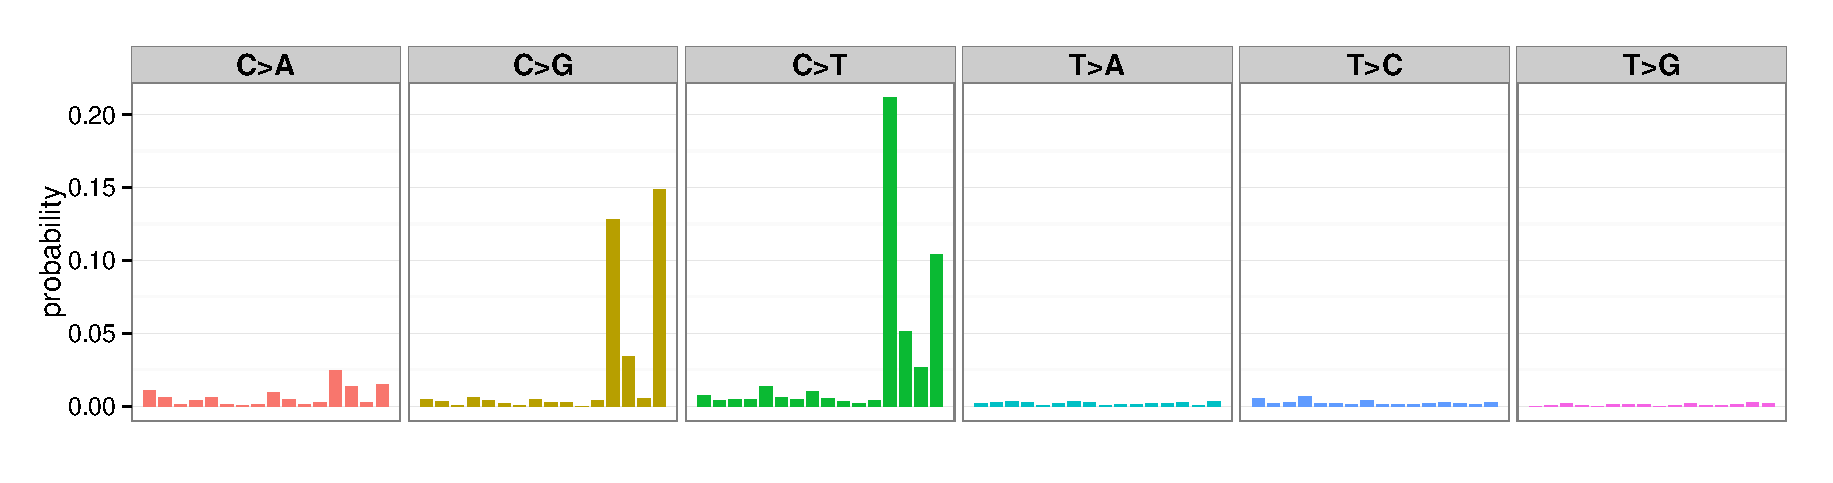
\includegraphics[width=15cm,height=4cm]{example96_APOBEC.eps}
  \label{APOBEC_nature2013_sig}}
  
\subfigure[POLE signature in the previous study]{%
  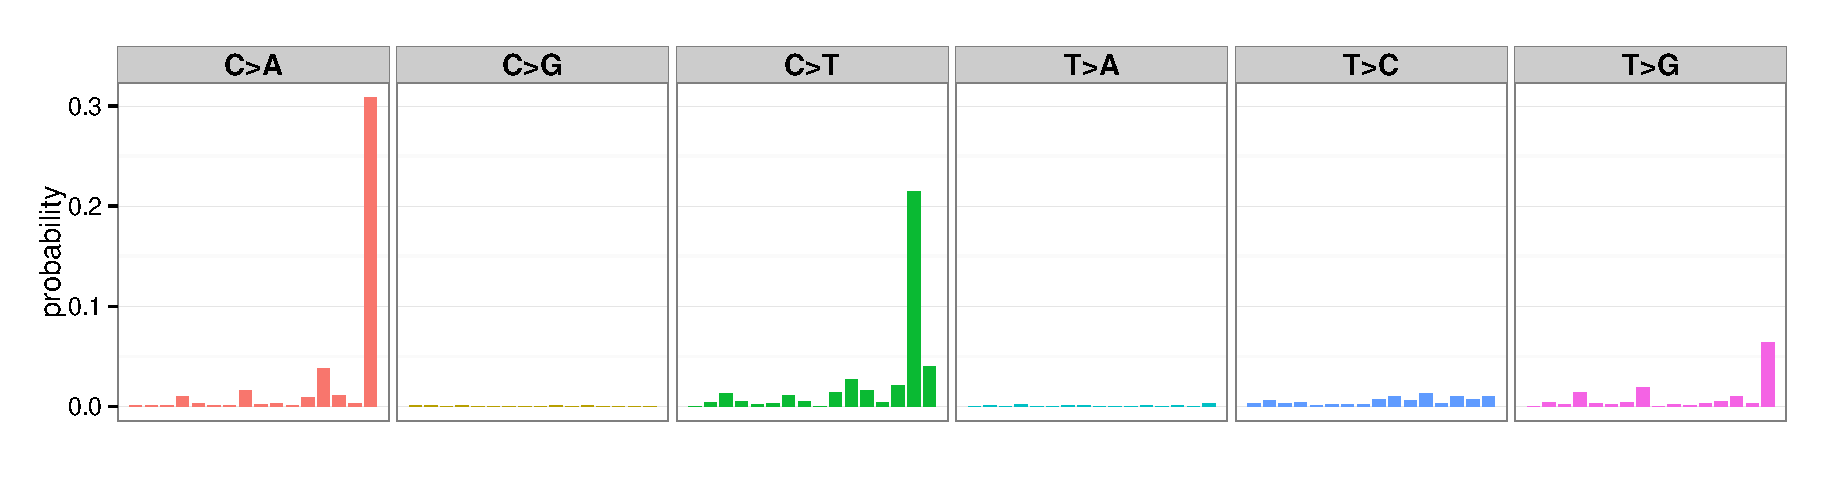
\includegraphics[width=15cm,height=4cm]{example96_POLE.eps}
  \label{POLE_nature2013_sig}}
  
\caption{The APOBEC and POLE signatures extracted in the previous study (Signature 2 and 10 in \cite{pmid23945592}, respectively).
The barplots are divided by 6 substitution patterns.
In each division, 16 bars show joint probabilities of 16 combinations of the immediate 5' and 3' bases  
(ApNpA, ApNpC, ApNpG, ApNpT, CpNpA, $\cdots$, TpTpT).
(a) The strong intensities of the last four bars for the three substitution patterns with original bases C 
indicates that the immediate 5' base is mostly confined to T in this signature.
Also, the frequency of the immediate 3' bases for the mutation patterns at TpCpN sites are mostly proportional across three major substitution patterns (C $>$ A, C $>$ G and C $>$ T).
(b) The strong intensities on TpCpT $>$ TpApT and TpCpG $>$ TpTpG are observed. This is a little complex in the sense that 
the immediate 3' base and the substitution pattern are not independent.
}
\label{nature2013_example}
\end{figure*}


\clearpage


\begin{figure*}

\begin{minipage}{0.6\textwidth}
\begin{center}
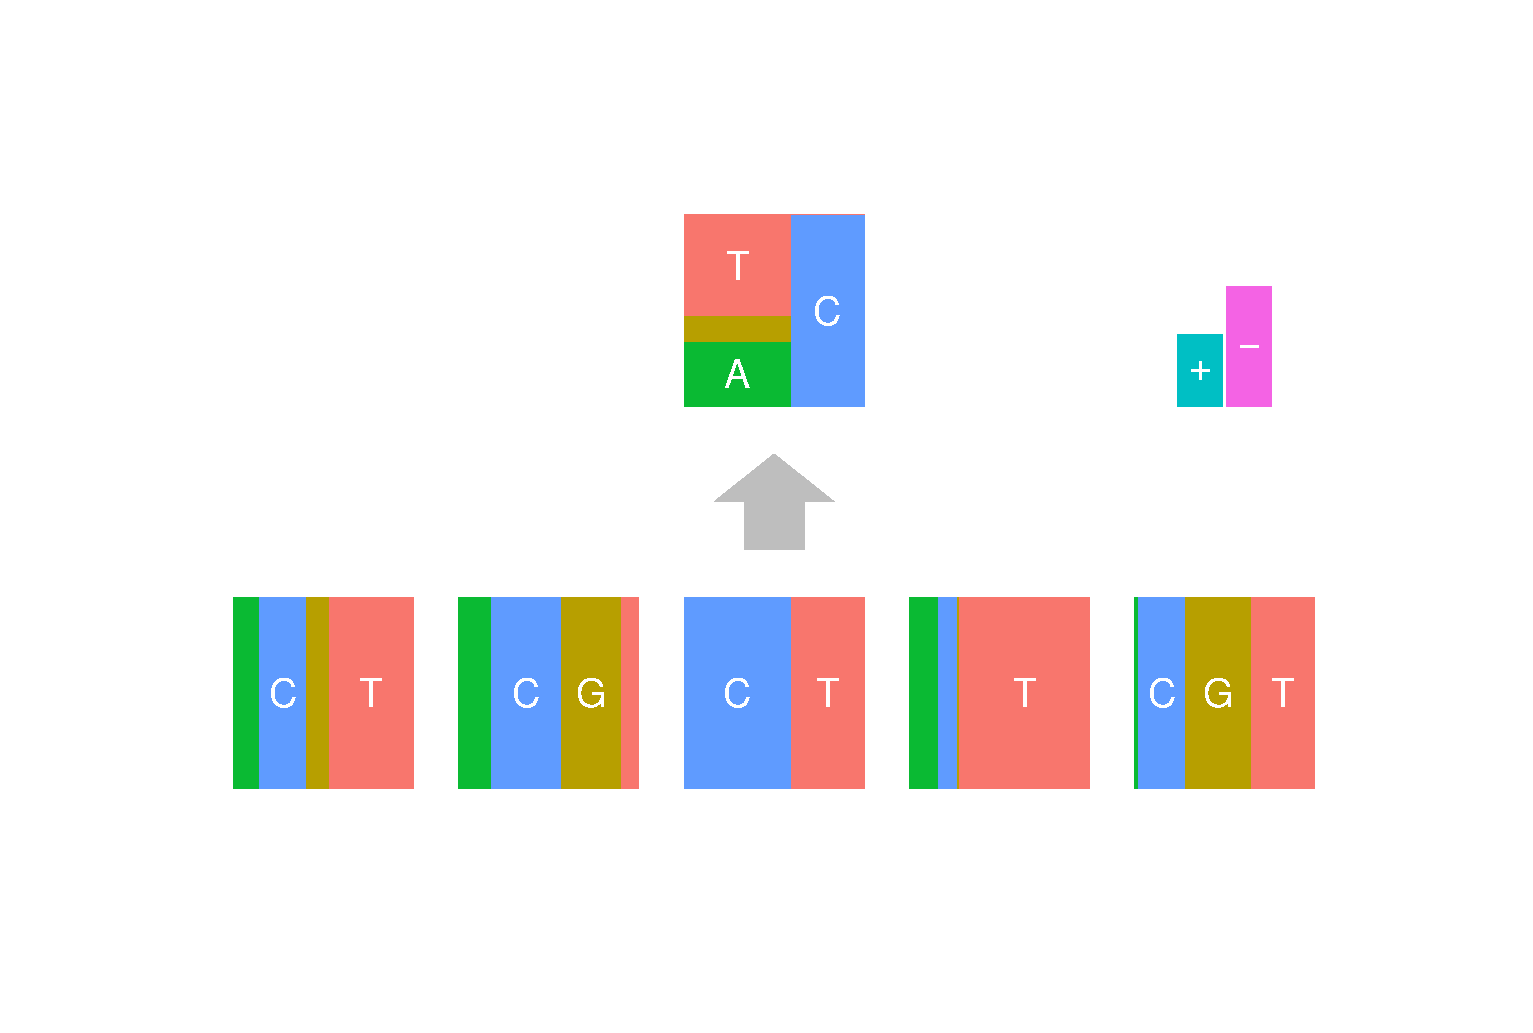
\includegraphics[width=10cm,height=6.66cm]{example_signature.eps}

\end{center}
\end{minipage}
\begin{minipage}{0.4\textwidth}

\begin{flushleft}
\makeatletter
 \def\@captype{table}
\makeatother

\subtable[substitution pattern]{\label{tab:tab11}
\footnotesize
\begin{tabular}{|c|c|c|c|c|c|}
\hline
C$>$A & C$>$G & C$>$T & T$>$A & T$>$C & T$>$G \\
\hline
0.201 & 0.080 & 0.314 & 0.000 & 0.405 & 0.000 \\
\hline
\end{tabular}
}

\subtable[adjacent bases]{\label{tab:tab12}
\footnotesize
\begin{tabular}{|c|c|c|c|c|}
\hline
position  & A & C &  G & T \\
\hline
-2 & 0.146 & 0.257 & 0.128 & 0.469 \\
-1 & 0.183 & 0.389 & 0.331 & 0.097 \\
+1 & 0.161 & 0.107 & 0.013 & 0.719 \\
+2 & 0.019 & 0.265 & 0.366 & 0.350 \\
\hline
\end{tabular}
}


\subtable[strand direction]{\label{tab:tab13}
\footnotesize
\begin{tabular}{|c|c|}
\hline
plus strand & minus strand  \\
\hline
0.375 & 0.625 \\
\hline
\end{tabular}
}

% \caption{sample}
% \label{label 2}
\end{flushleft}
\end{minipage}
\caption{An example of a mutation signature and its visualization in the proposed approach.
Here, mutation features (substitution patterns, two 5' and 3' bases and strand direction) 
are assumed to be independent ($L=6$, $\bm{M} = (6, 4, 4, 4, 4, 2)$).
In the bottom, the size of each box represents the frequencies of bases (A, C, G and T) at the flanking sites.
In the top, the height of each box represents the conditional frequencies of mutated bases for each original base (C and T).
In the upper right, the height of the $+$ box represents the frequencies of mutations in the coding strand (or the plus strand, the sense strand and the untranscribed strand)
whose nucleotide sequences directly corresponds to mRNA, 
whereas the height of $-$ box represents those in the template strand (or the minus strand, the antisense strand, the transcribed strand and the noncoding strand)
whose sequences are copied during the synthesis of mRNA.
}
\label{mutSig_example}

\end{figure*}


\clearpage


\begin{figure*}
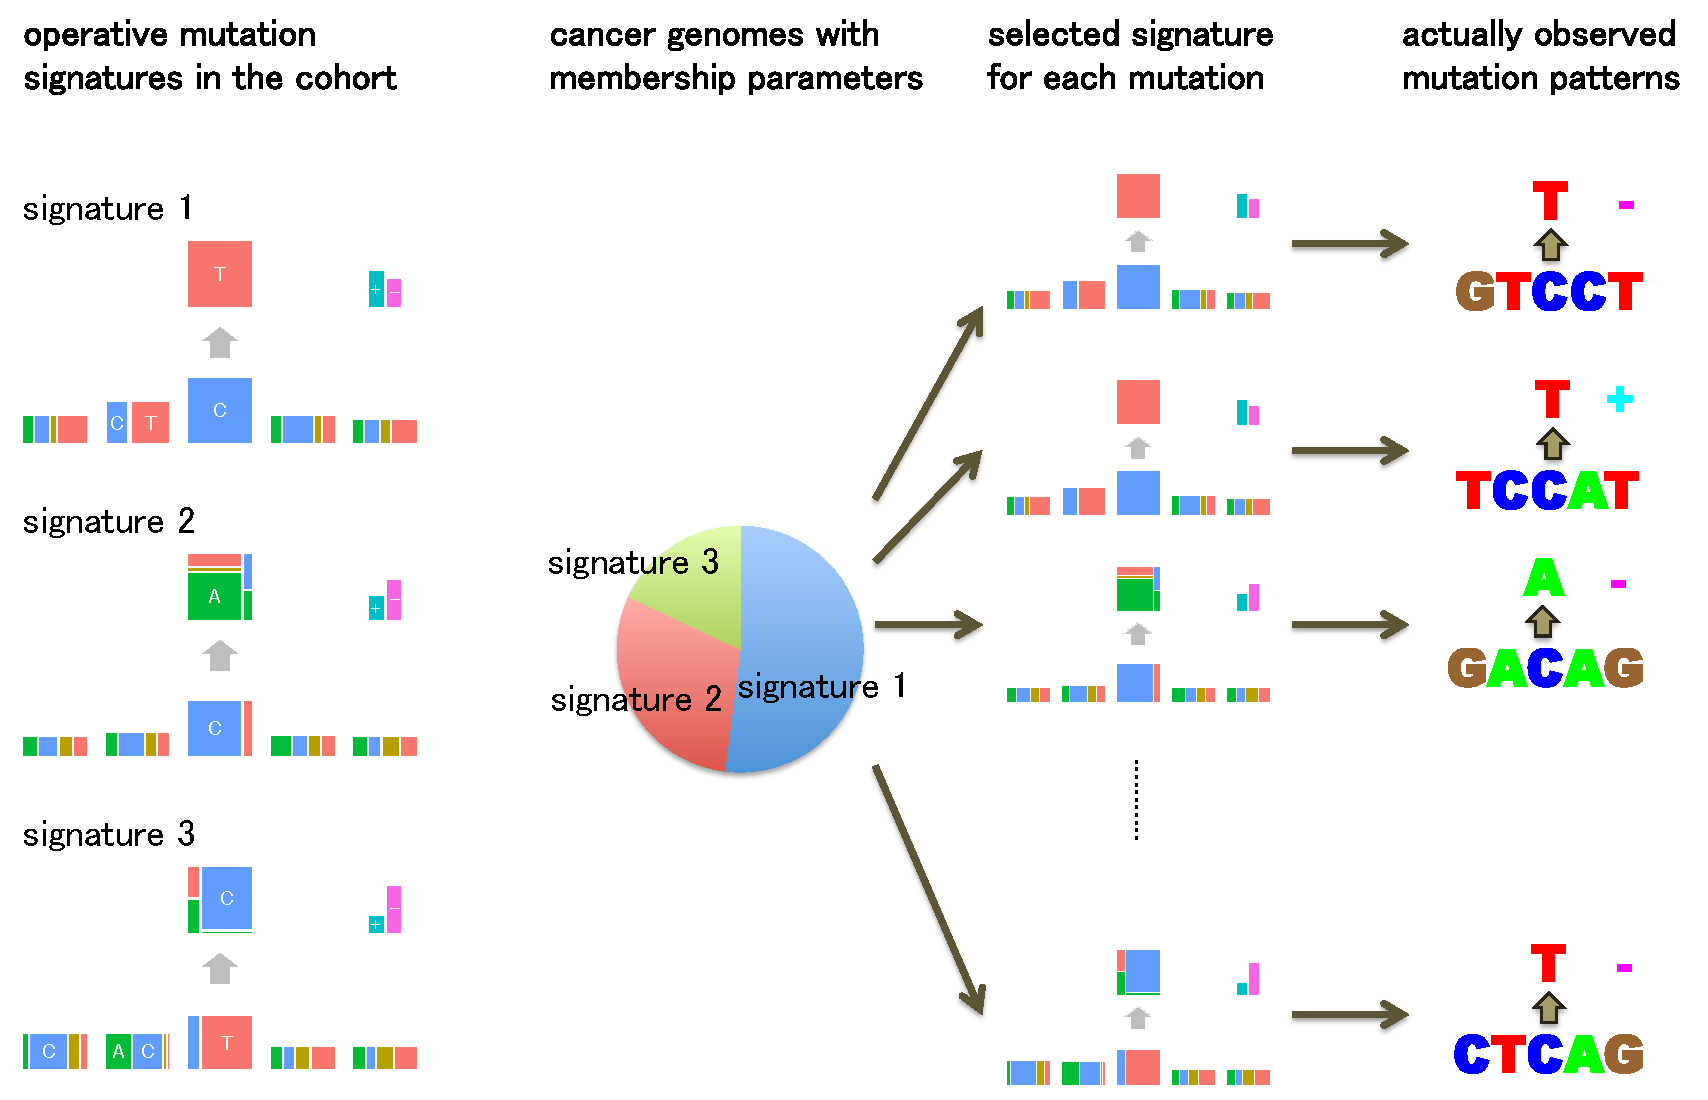
\includegraphics[width=450pt]{methodOverview.pdf}
\caption{Suppose there are three types of mutation sources (mutation signatures) such as ultraviolet, tobacco smoking chemicals and transcription coupled repairs.
Each cancer genome has ratios showing which types of mutation sources are contributing to its mutations (membership parameters).
The generative model of the pattern of each mutation is:
first, one of the mutation signatures is chosen according to the membership parameter.
Second, according to the selected mutation signature, mutation features such as substitution pattens and flanking bases are generated 
by the corresponding multinomial distributions for that mutation signature.
}
\label{methodOverview}
\end{figure*}



\clearpage

\begin{figure*}[b]
\centering
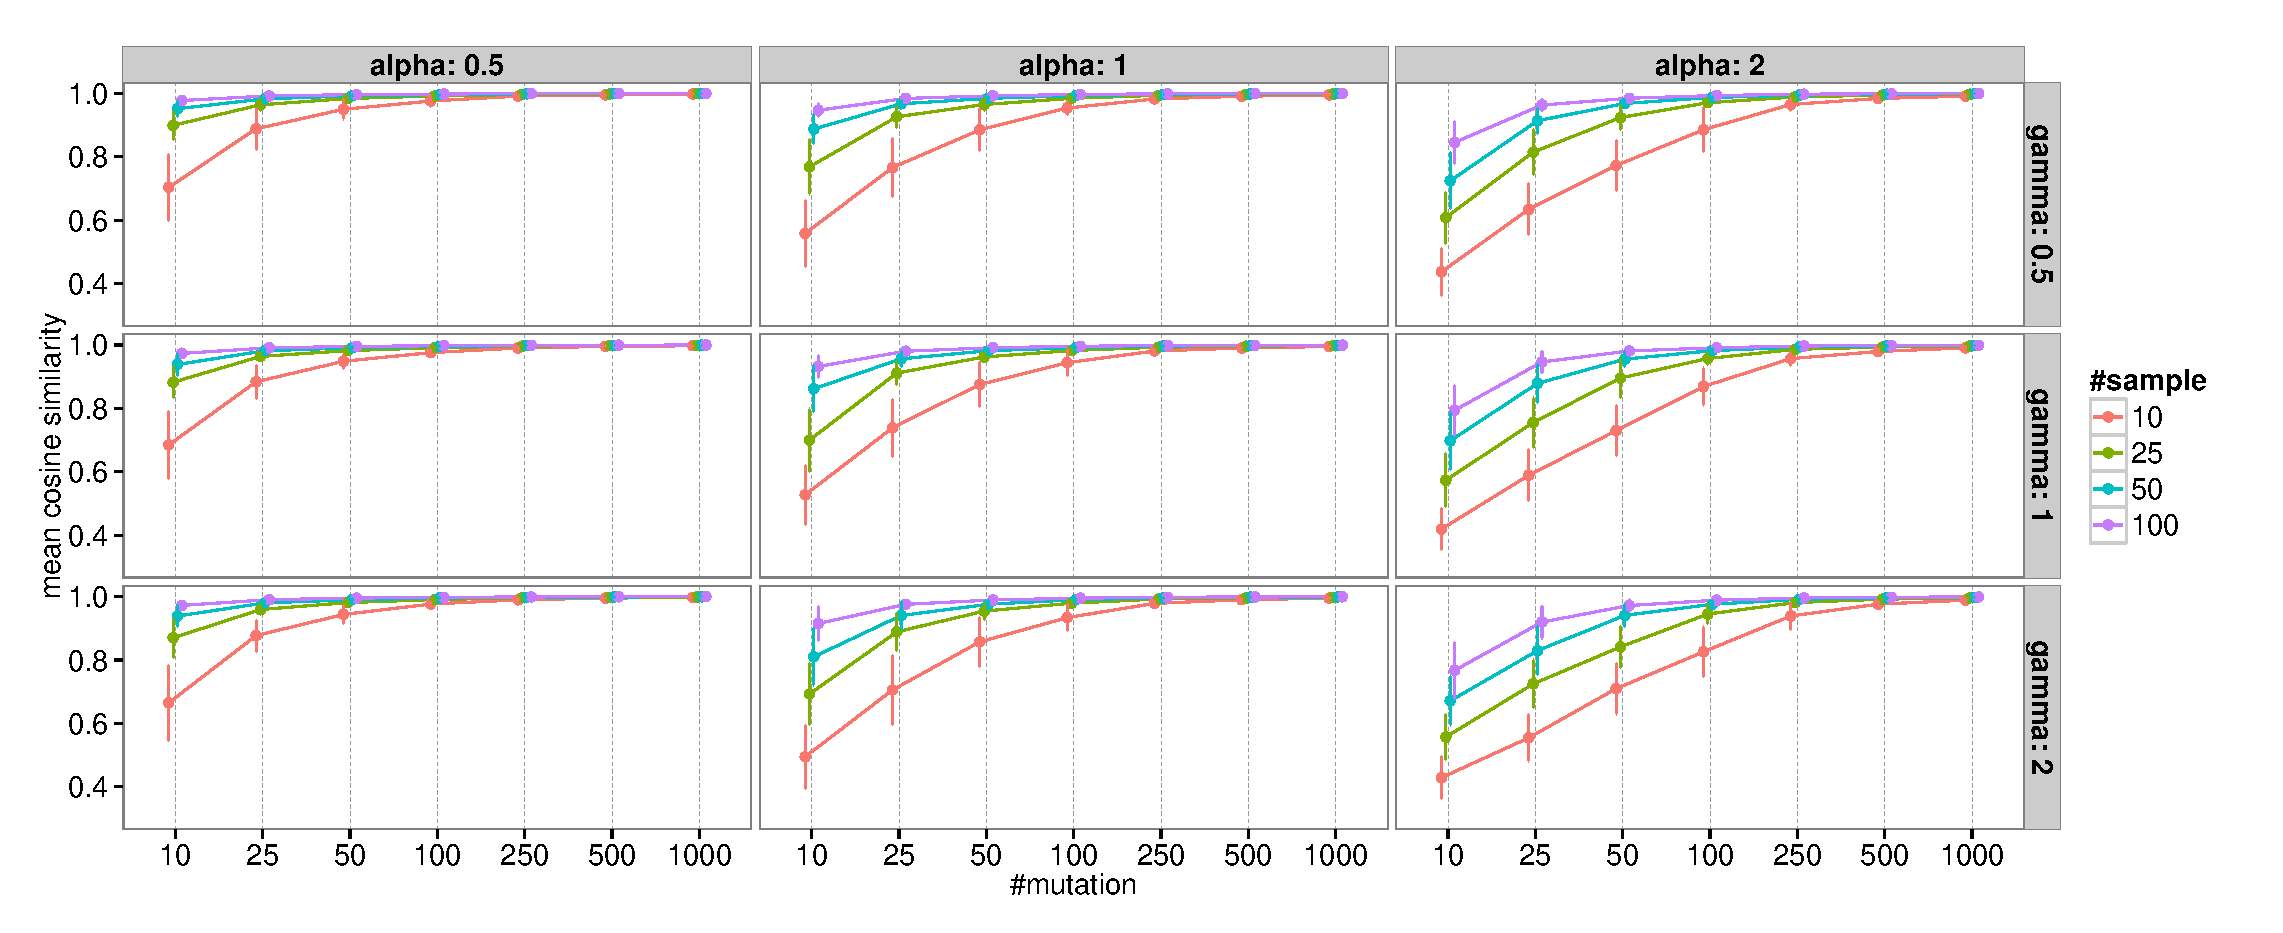
\includegraphics[width=16cm,height=6cm]{simulation_result.eps}
\caption{The accuracy of the proposed approach for the simulated data 
when changing the number of samples, mutations, 
and the amounts of dispersion parameters ($\alpha$ and $\gamma$) for the mutation features and signature distribution parameters.
}
\label{sim_facet}
\end{figure*}



\begin{figure*}[ht]
\centering

\subfigure[APOBEC signature for the independent model]{%
  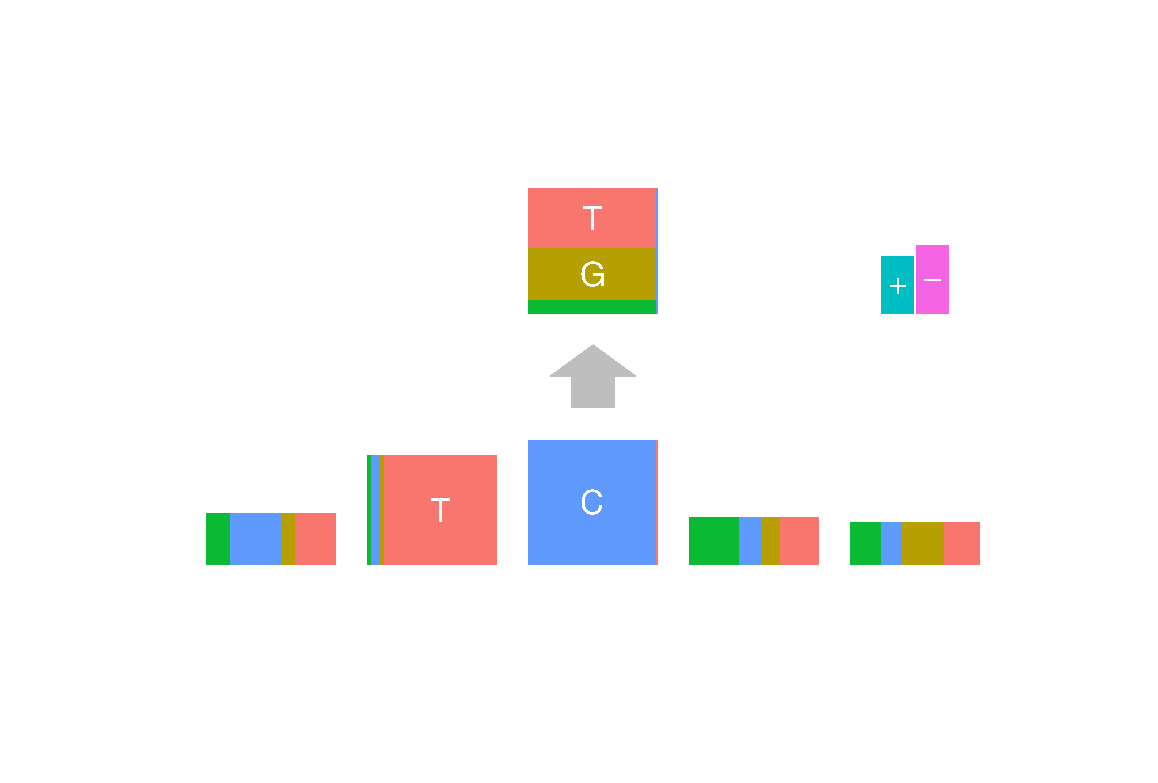
\includegraphics[height=5cm,width=7.5cm,clip]{UTUC_APOBEC_ind.eps}
  \label{UTUC:APOBEC_ind5_sig}}
\quad
\subfigure[AA signature for the independent model]{%
  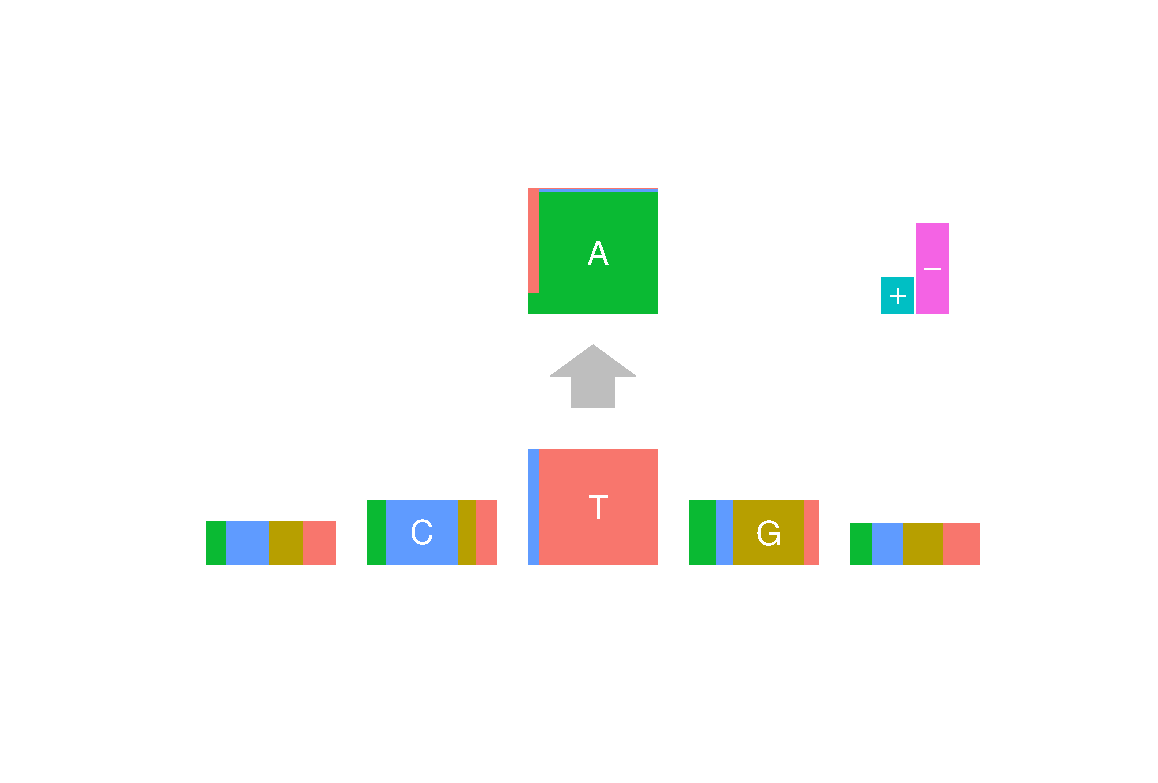
\includegraphics[height=5cm,width=7.5cm,clip]{UTUC_AA_ind.eps}
  \label{UTUC:AA_ind5_sig}}
  
  \subfigure[APOBEC signature for the full model]{%
  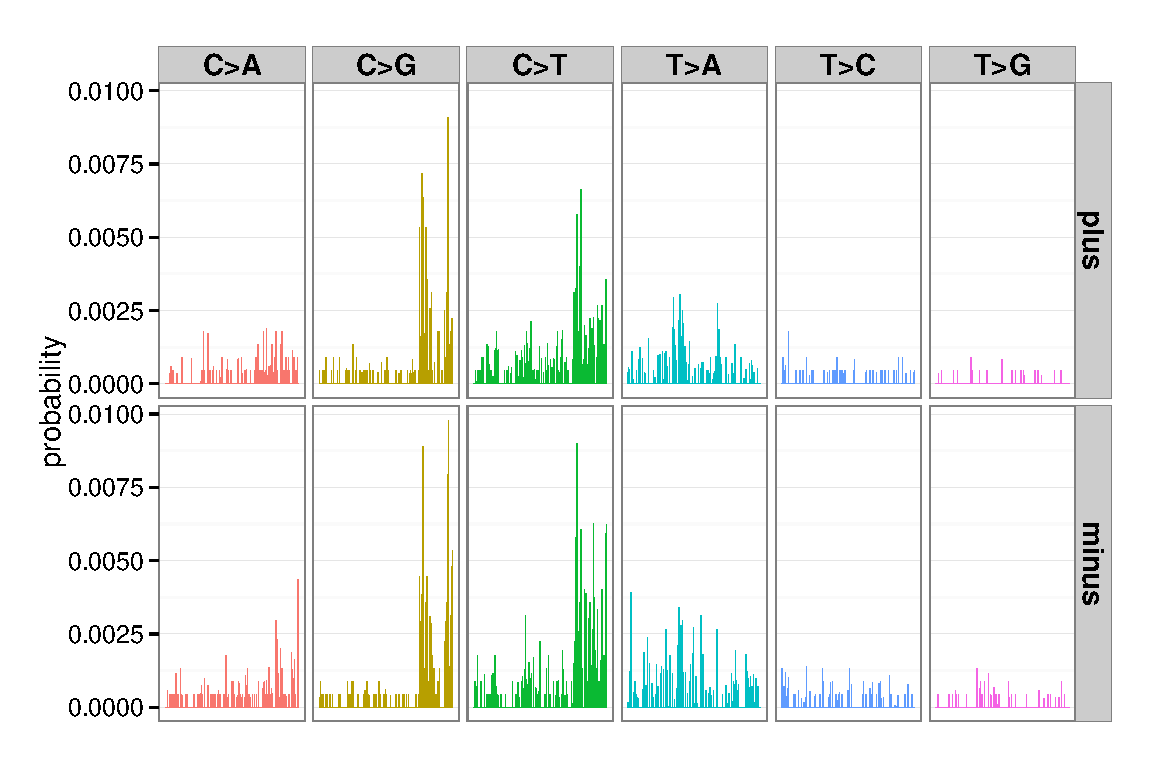
\includegraphics[height=5cm,width=7.5cm,clip]{UTUC_APOBEC_full.eps}
  \label{UTUC:APOBEC_full5_sig}}
\quad
\subfigure[AA signature for the full model]{%
  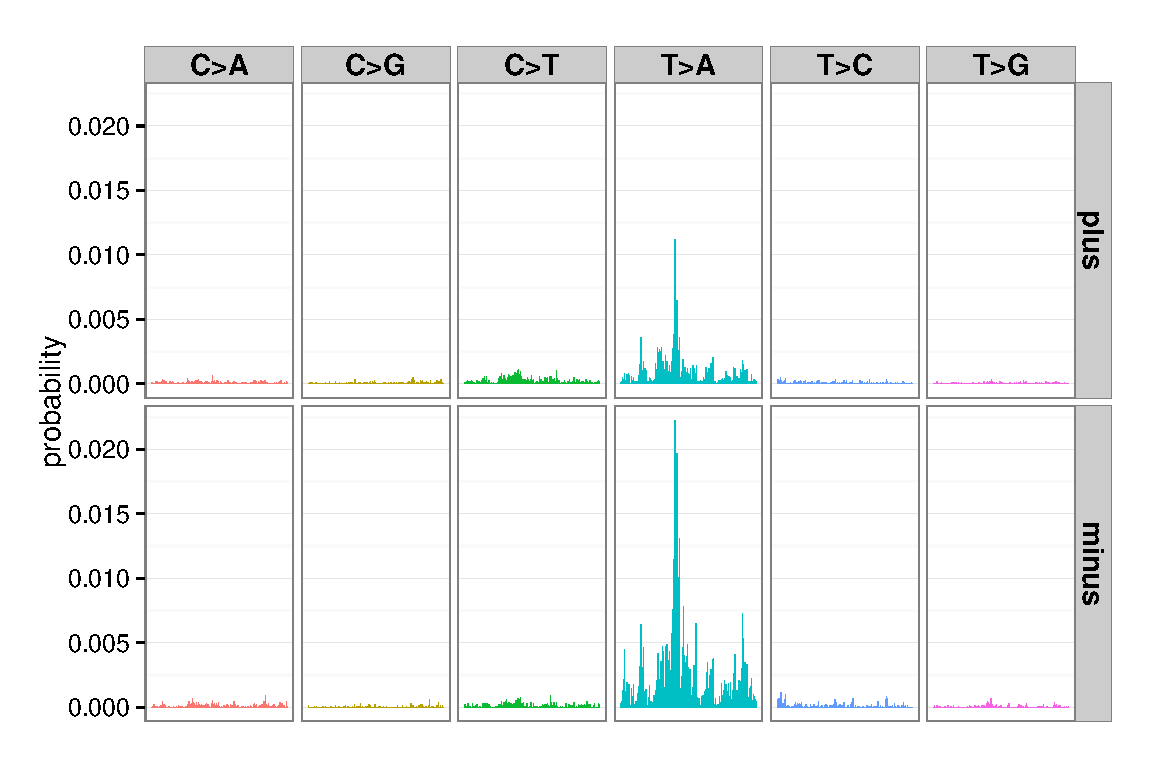
\includegraphics[height=5cm,width=7.5cm,clip]{UTUC_AA_full.eps}
  \label{UTUC:AA_full5_sig}}
  
\subfigure[APOBEC signature stability]{%
  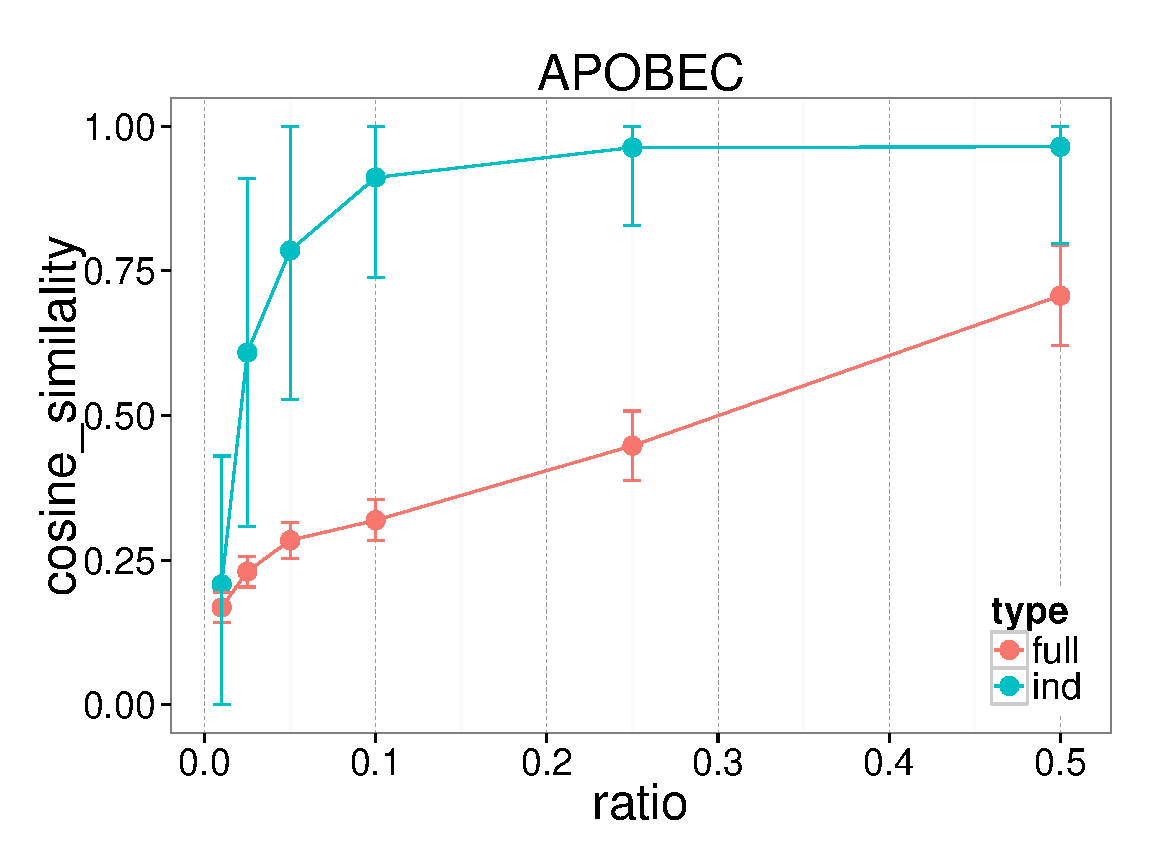
\includegraphics[height=5.5cm,width=7.5cm,clip]{UTUC_downsampling_APOBEC.eps}
  \label{UTUC:APOBEC_downsampling}}
\quad
\subfigure[AA signature stability]{%
  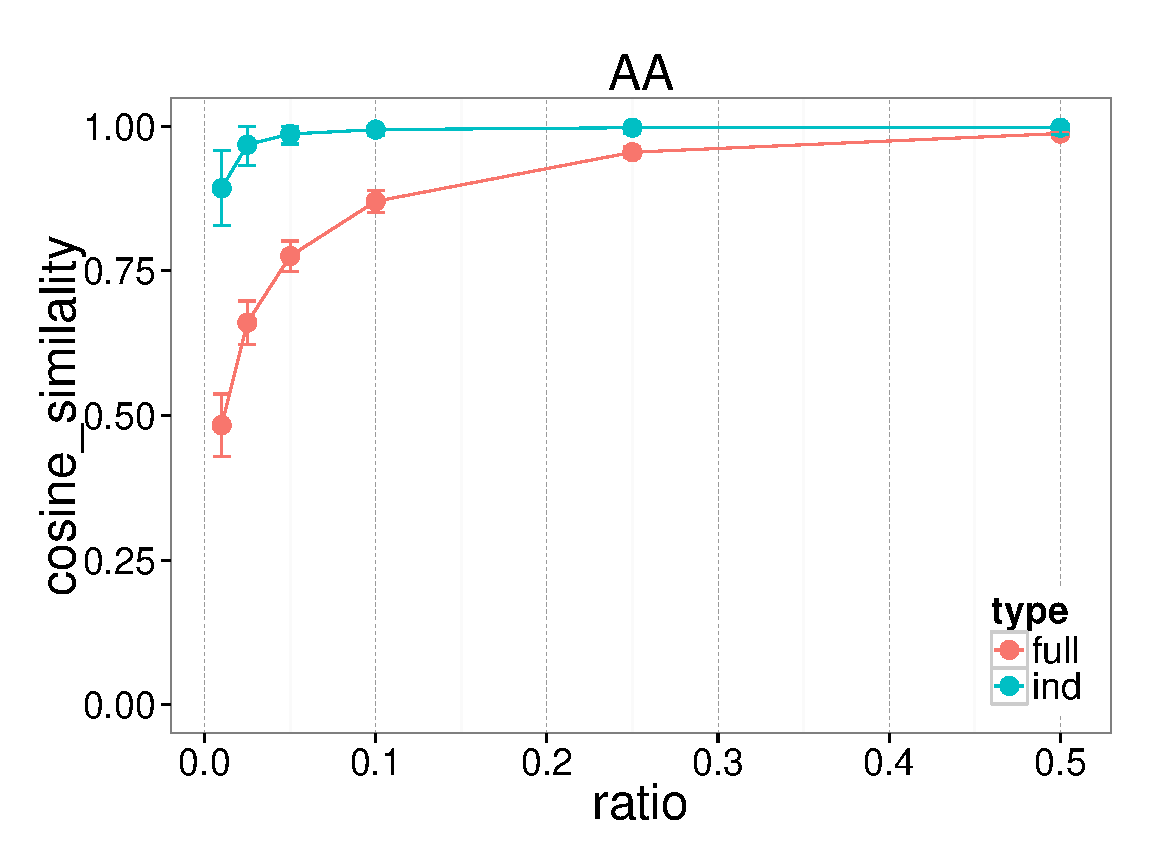
\includegraphics[height=5.5cm,width=7.5cm,clip]{UTUC_downsampling_AA.eps}
  \label{UTUC:AA_downsampling}}
%
\caption{The mutation signatures for the UTUC data, and the results of downsampling experiments. 
3072 elements in the full model mutation signatures were shown divided by 6 substitution patterns and strand directions.}
\label{UTUC}
\end{figure*}


\clearpage

\begin{figure*}[b]
\centering
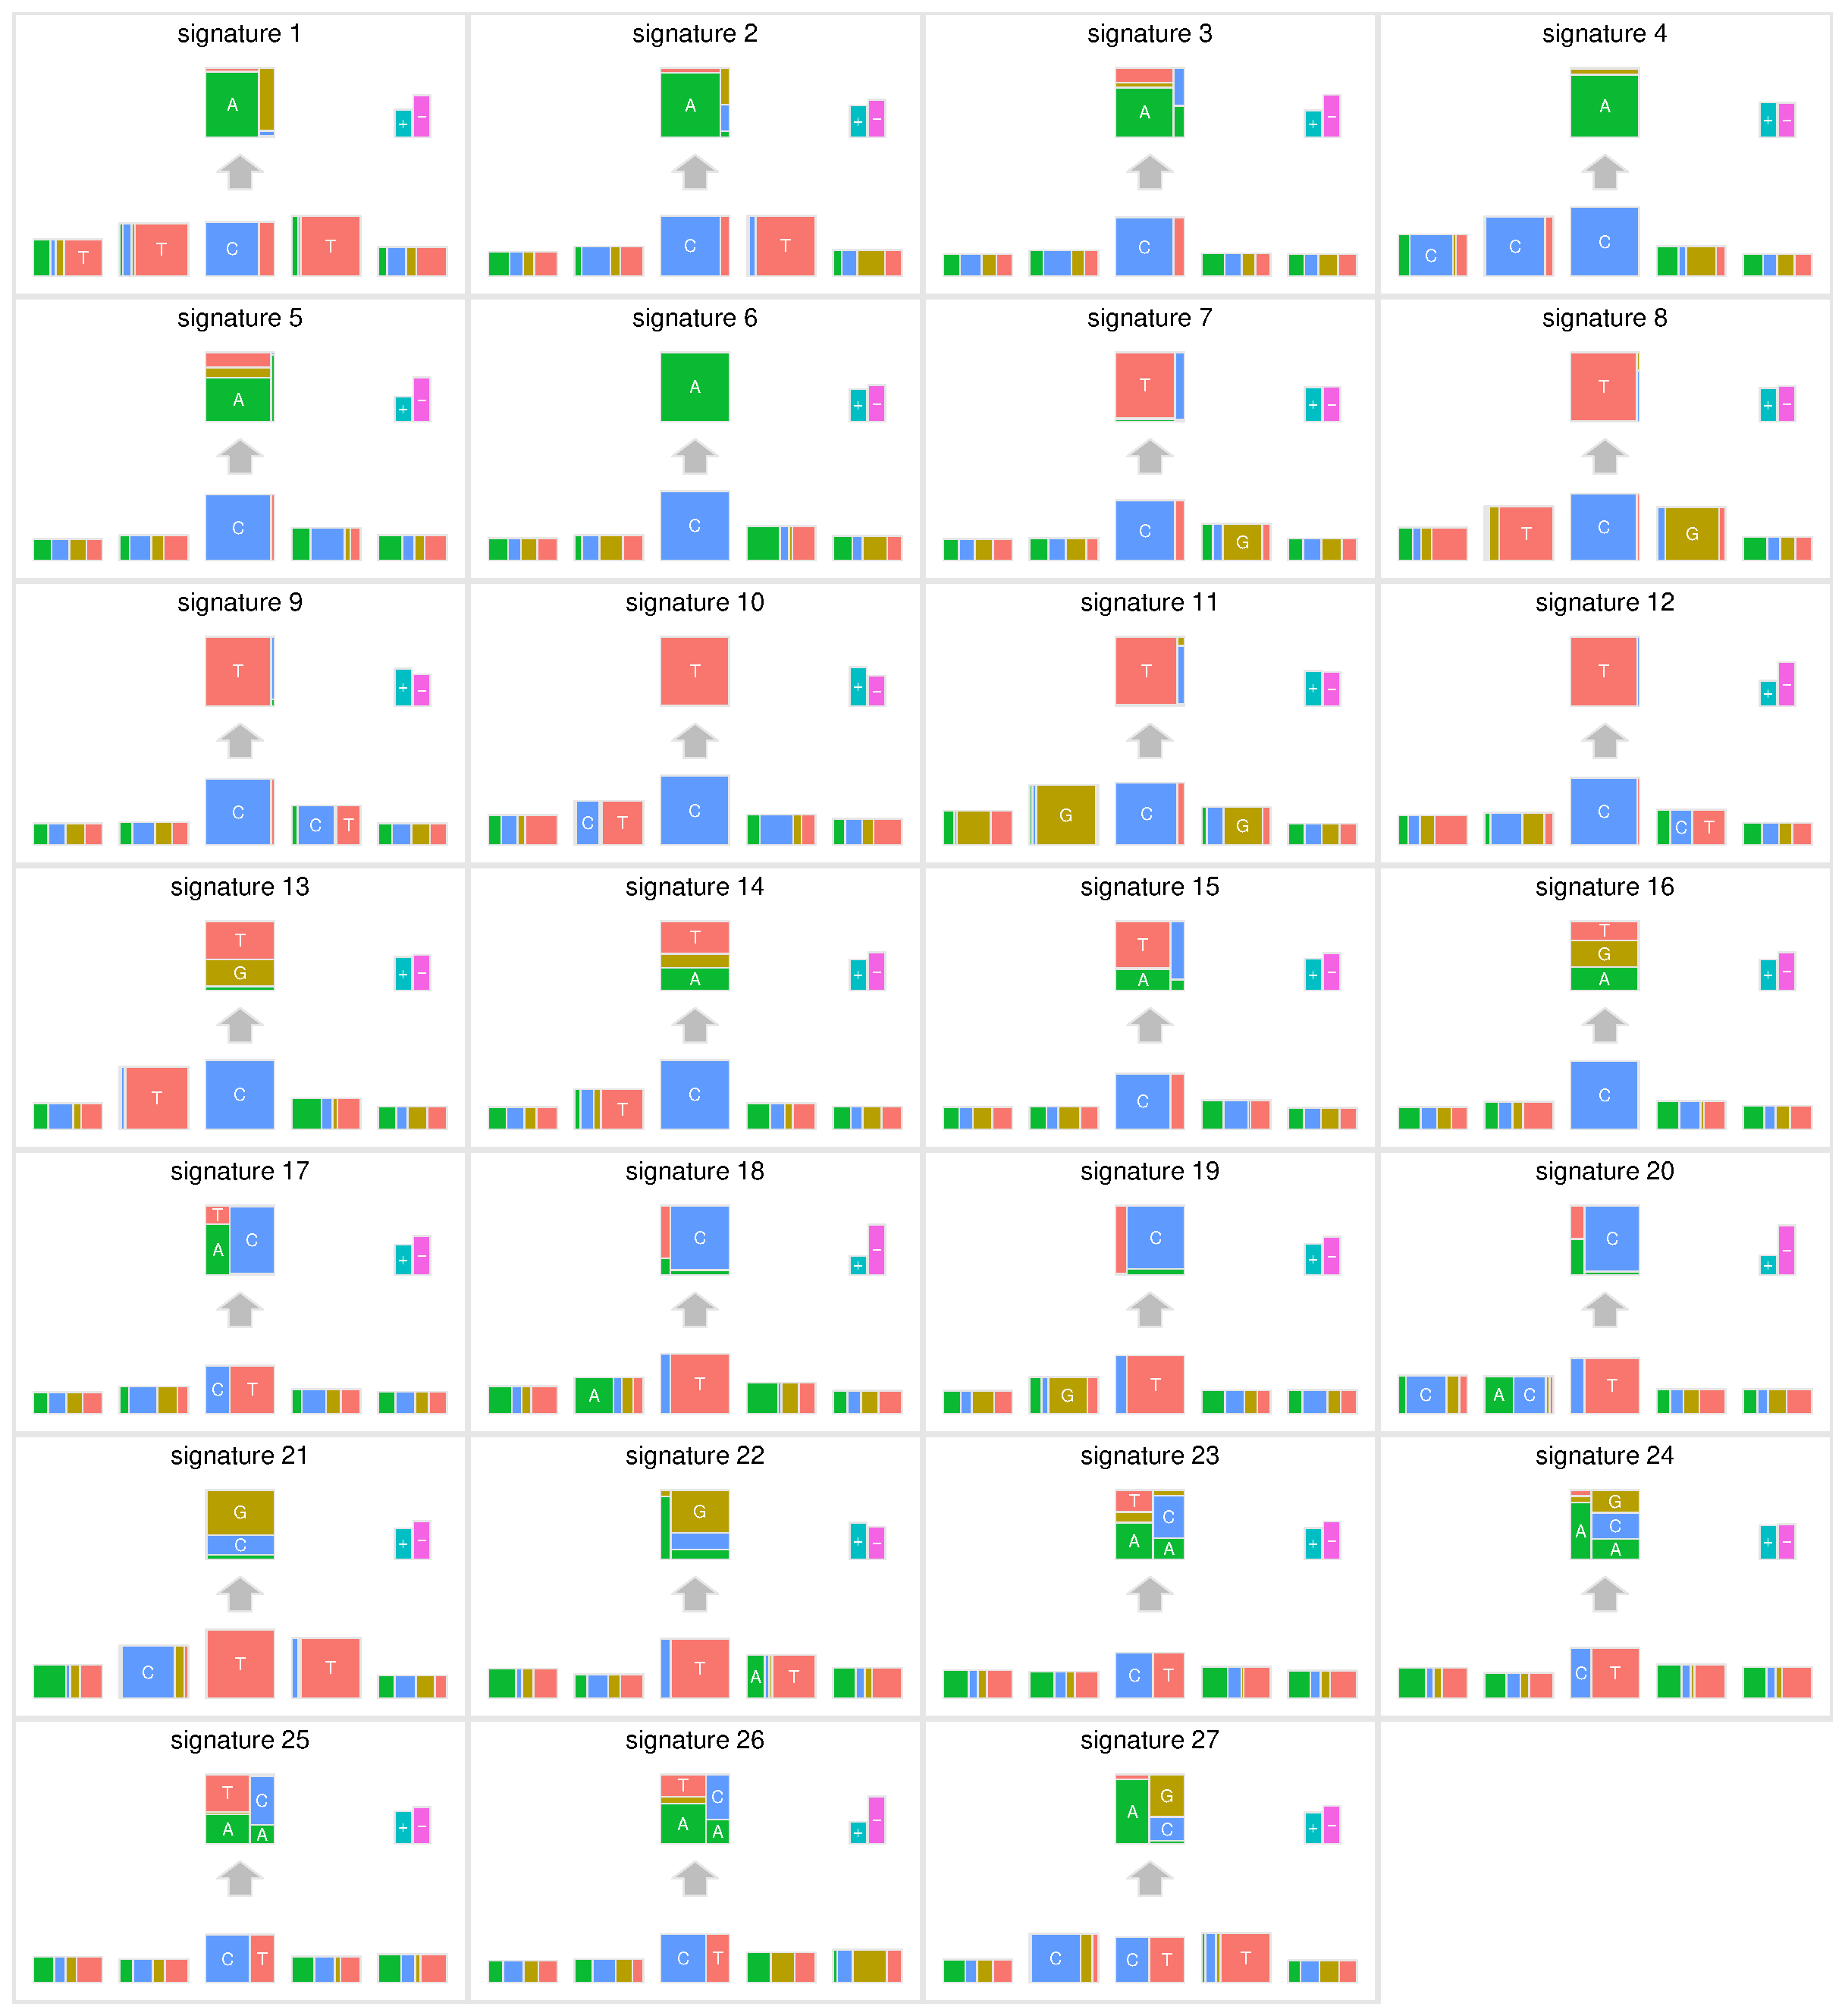
\includegraphics[width=16cm,height=17.5cm]{AlexandrovEtAl_mergedSignature.eps}
\caption{The summary of mutation signatures obtained in a reanalysis of the data of the previous study \cite{pmid23945592} using the proposed method,
where the substitution patterns and two 5' and 3' bases from the mutated sites are taken into account as mutation features.
First, the mutation signatures were estimated with respect to each cancer type,
then the similar signatures (the sum of the square distances between the parameters is below 0.6) emerged across different cancer types were merged.
}
\label{nature2013_sig_summary}
\end{figure*}

\clearpage

\begin{figure*}[b]
\centering
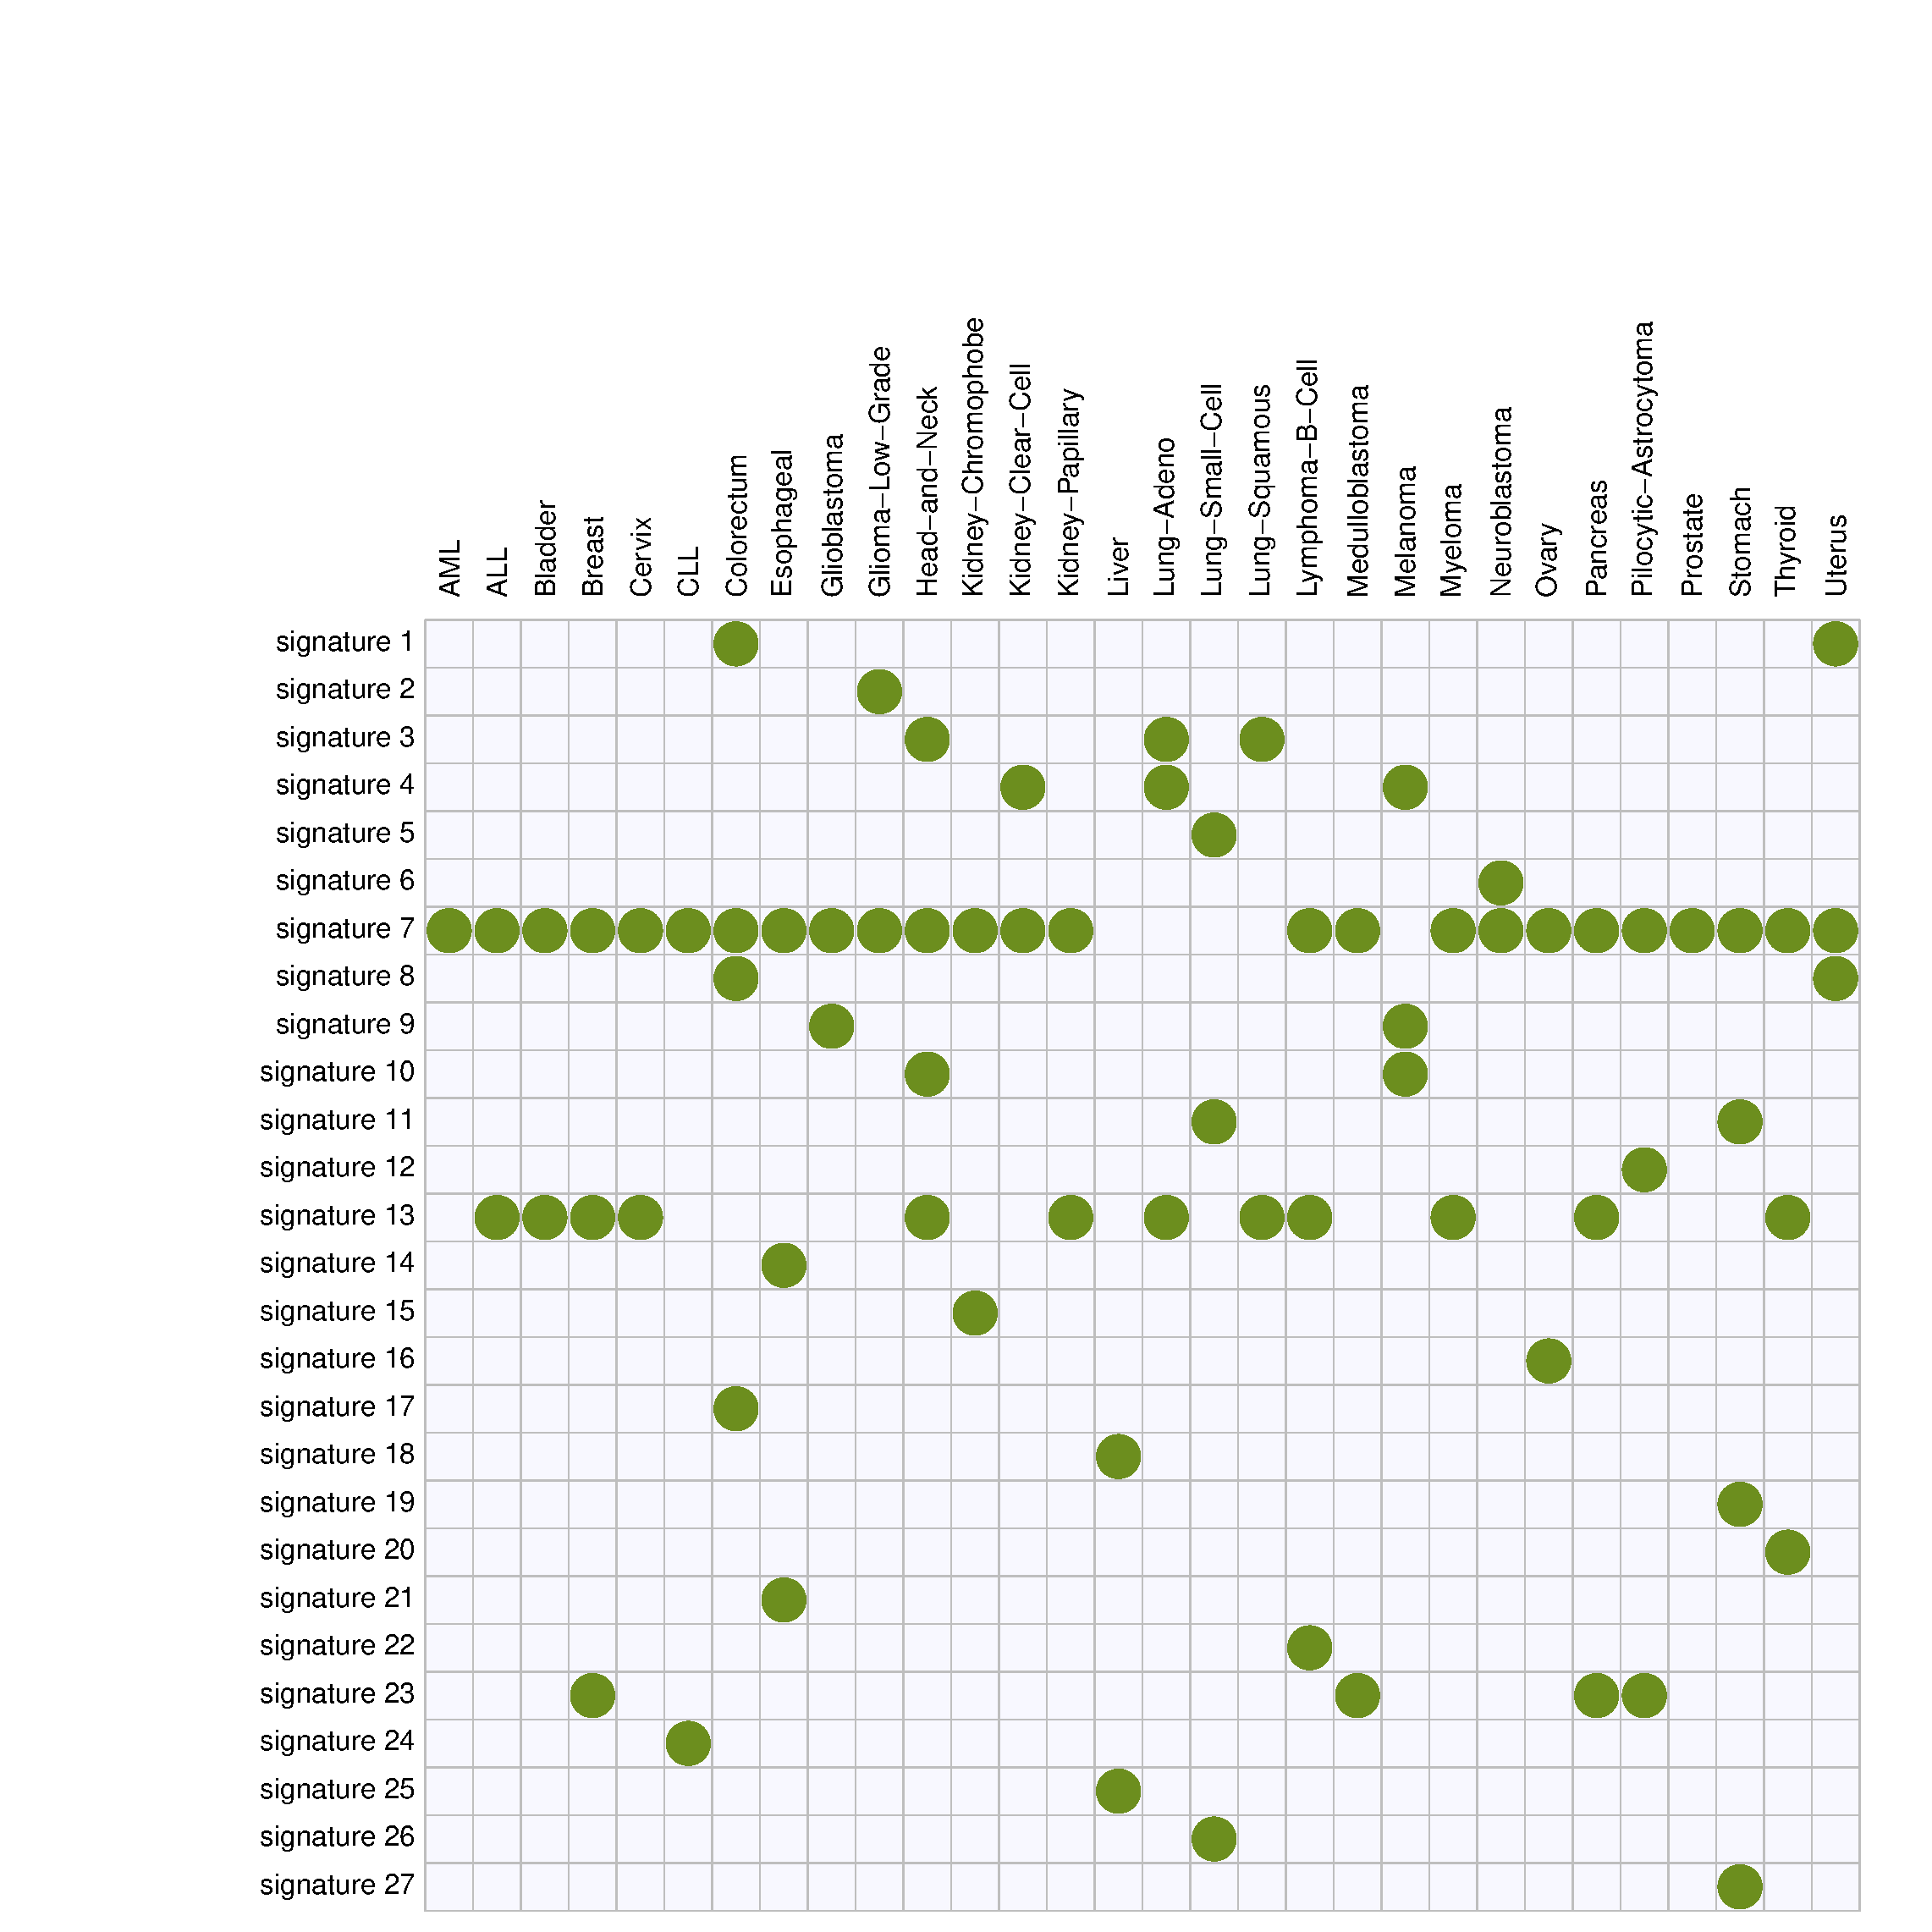
\includegraphics[width=15cm,height=15cm]{corrplot.eps}
\caption{The summary of membership of each mutation signature across 30 cancer types obtained using the proposed method.}
\label{nature2013_sig_member}
\end{figure*}


\clearpage



% \begin{figure*}[b]

\begin{figure*}[b]

\subfigure[APOBEC signature intensities at two 5' to the mutated site]{%
  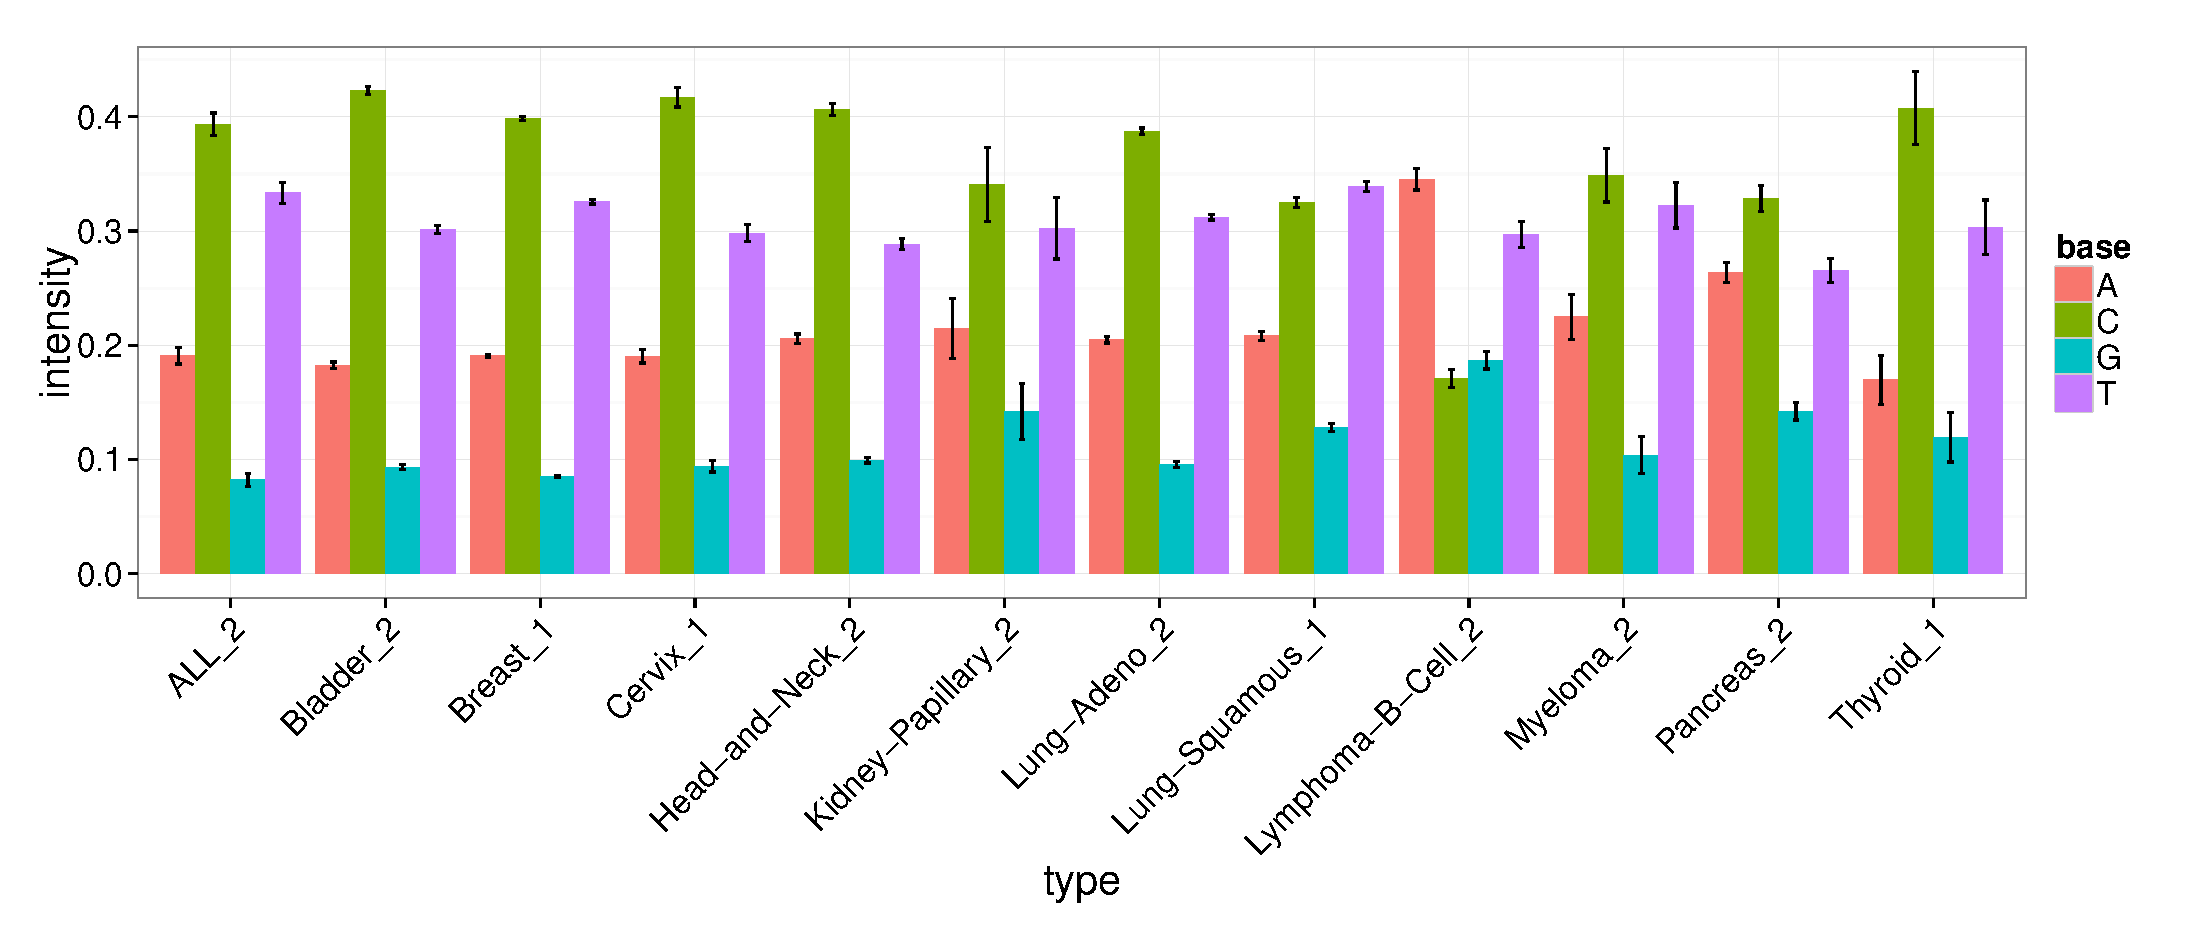
\includegraphics[width=14.5cm,height=6cm]{APOBEC_two5prime.eps}
   \label{APOBEC_two5prime}}
  
\subfigure[POLE1 signature intensities at two 5' to the mutated site]{%
  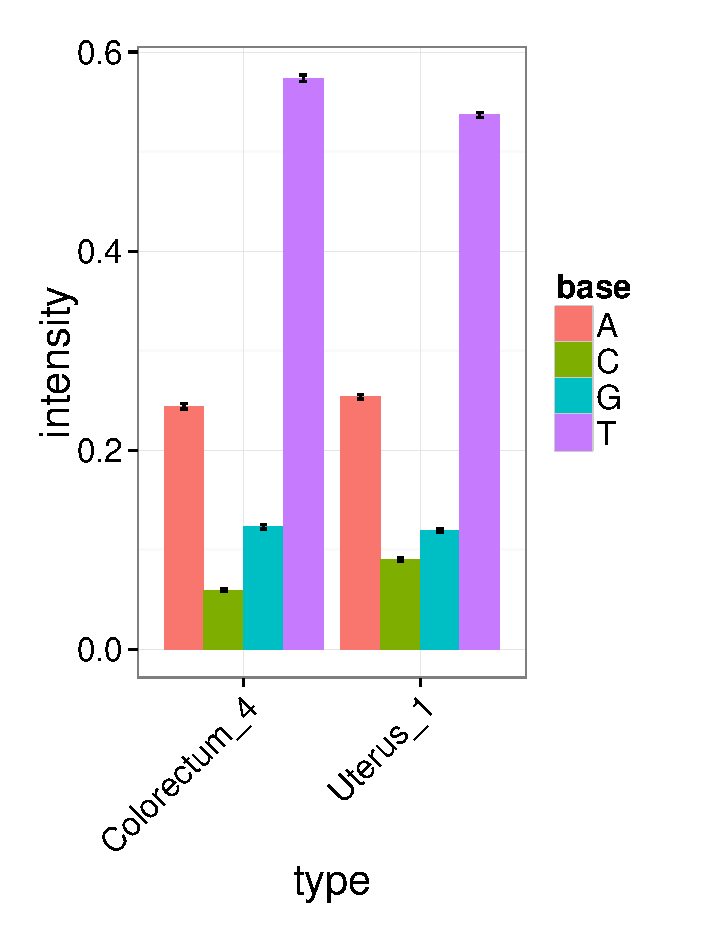
\includegraphics[width=4.5cm,height=6cm]{POLE1_two5prime.eps}
  \label{POLE1_two5prime}}
\quad
\subfigure[POLE2 signature intensities at two 5' to the mutated site]{%
  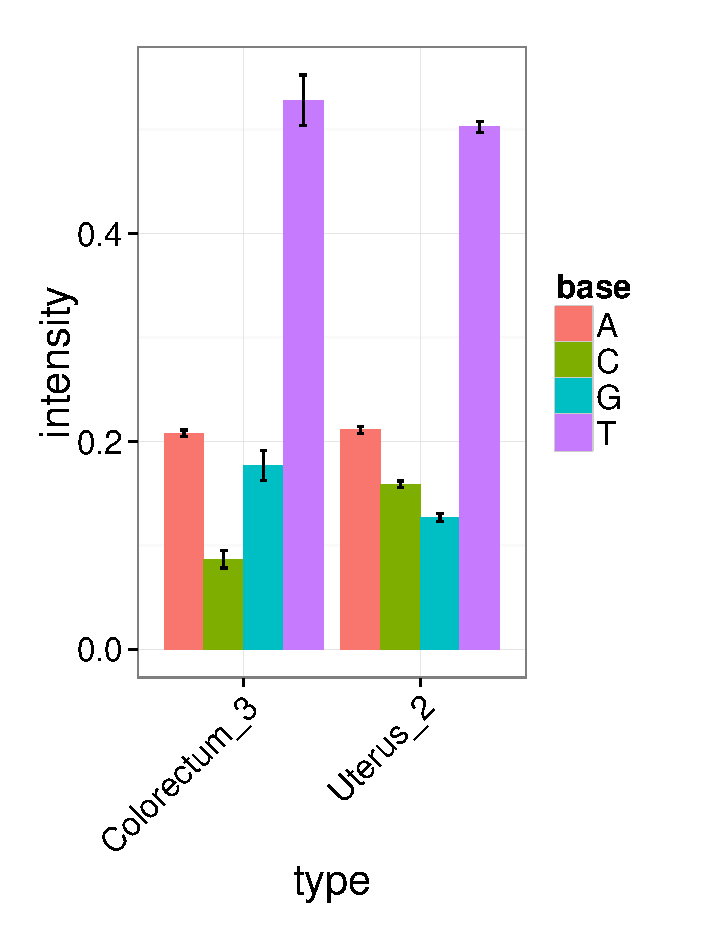
\includegraphics[width=4.5cm,height=6cm]{POLE2_two5prime.eps}
  \label{POLE2_two5prime}}

\subfigure[UV signature intensities at two 5' to the mutated site]{%
  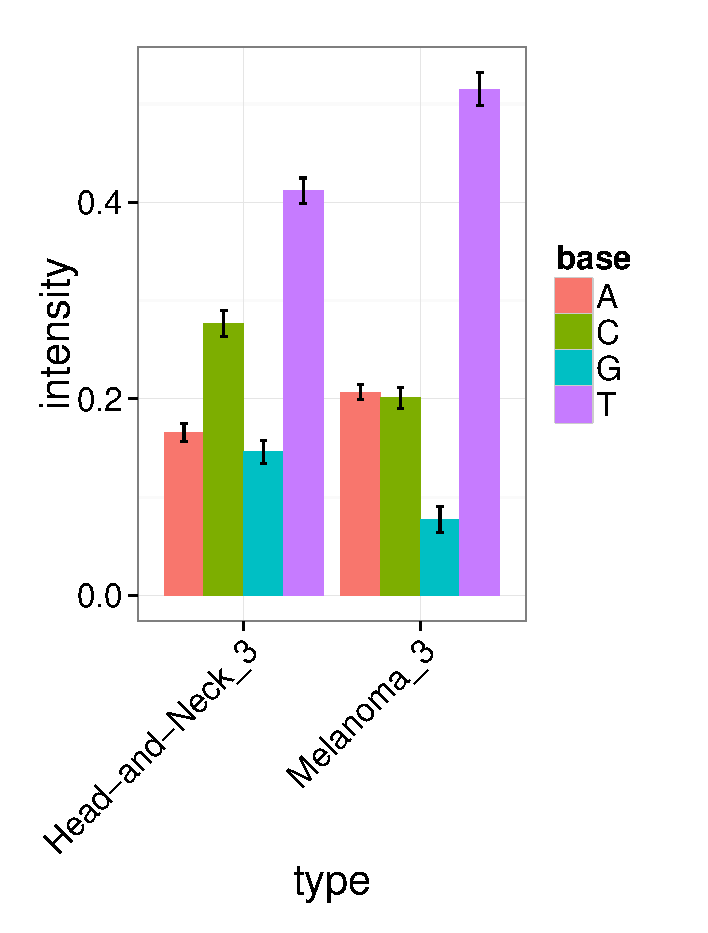
\includegraphics[width=4.5cm,height=6cm]{UV_two5prime.eps}
  \label{UV_two5prime}}
\quad
\subfigure[The signature 11 intensities at two 5' to the mutated site]{%
  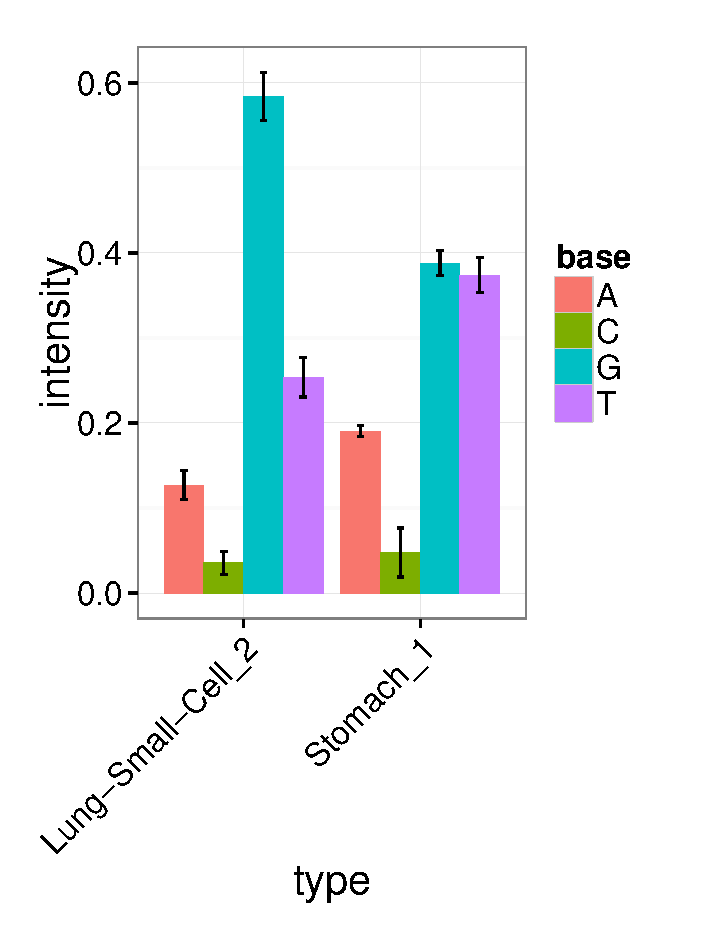
\includegraphics[width=4.5cm,height=6cm]{LMST_two5prime.eps}
  \label{LMST_two5prime}}
  
\caption{The estimated frequencies of bases at two 5' to the mutated site for each cancer type.
The heights of bar show the estimated frequency for bases A, C, G and T at two 5' to the mutated site.
The error bars show standard errors estimated by bootstrap.}
\label{two5prime}

\end{figure*}

% \begin{figure*}[b]

% \subfigure[POLE1 signatures in each cancer type]{%
%  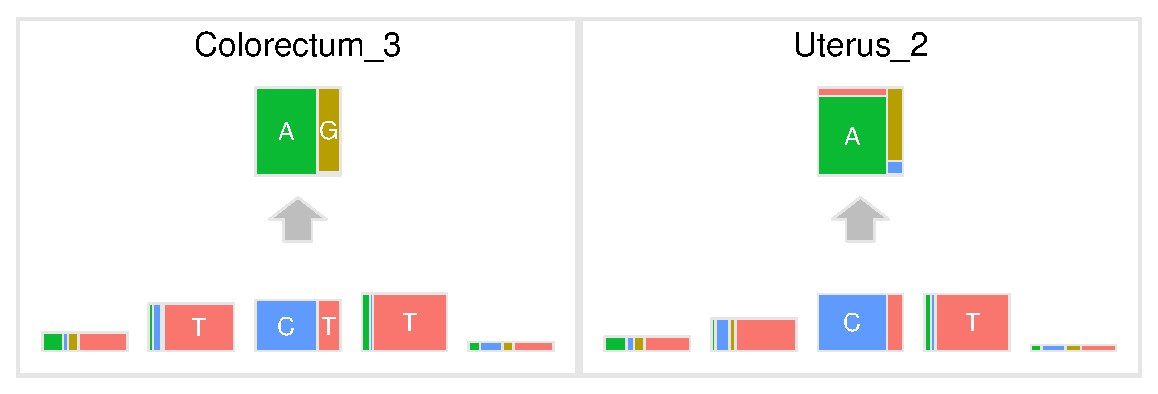
\includegraphics[width=7.5cm,height=2.5cm]{signatureList_POLE1.eps}
%   \label{POLE1_sig_list}}
  
% \subfigure[POLE2 signature in each cancer type]{%
%   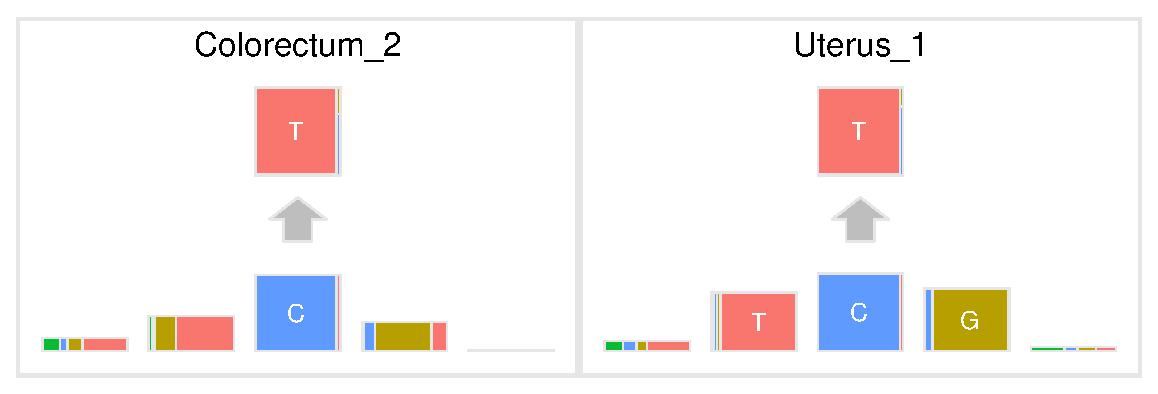
\includegraphics[width=7.5cm,height=2.5cm]{signatureList_POLE2.eps}
%   \label{POLE2_sig_list}}
  
% \subfigure[UV signature in each cancer type]{%
%   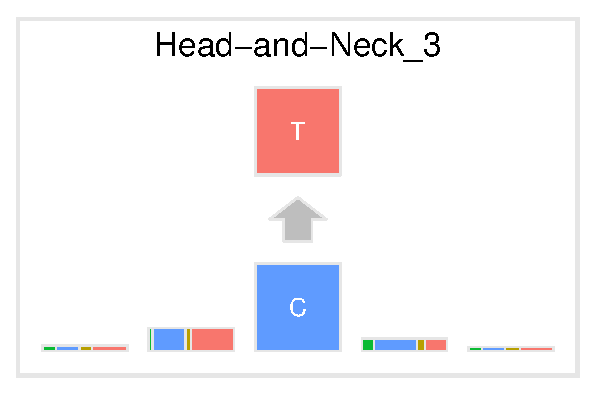
\includegraphics[width=7.5cm,height=2.5cm]{signatureList_UV.eps}
%   \label{UV_sig_list}}

% \subfigure[Unknown signature obtained in lung small cell carcinomas and stomach cancers]{%
%   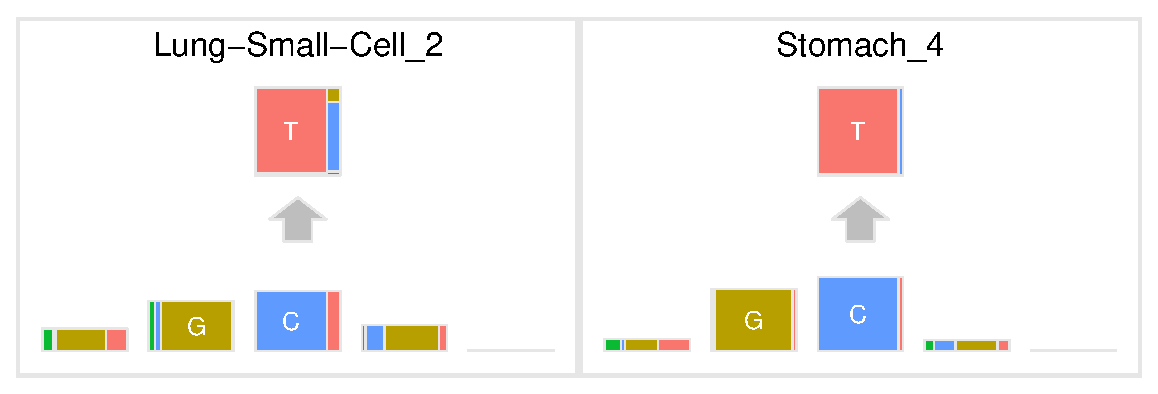
\includegraphics[width=7.5cm,height=2.5cm]{signatureList_LMST.eps}
%   \label{LMST_sig_list}}
      
% \caption{Several signatures having prominent characteristics at 5'  or 3' to the mutated sites.}
% \label{nature2013_sig_others}
% \end{figure*}


% \section*{Supporting Information Legends}
%
% Please enter your Supporting Information captions below in the following format:
%\item{\bf Figure SX. Enter mandatory title here.} Enter optional descriptive information here.
% 
%\begin{description}
%\item {\bf}
%\item {\bf}
%\end{description}


\end{document}

